% Options for packages loaded elsewhere
\PassOptionsToPackage{unicode}{hyperref}
\PassOptionsToPackage{hyphens}{url}
%
\documentclass[
  man, noextraspace,floatsintext]{apa6}
\usepackage{lmodern}
\usepackage{amssymb,amsmath}
\usepackage{ifxetex,ifluatex}
\ifnum 0\ifxetex 1\fi\ifluatex 1\fi=0 % if pdftex
  \usepackage[T1]{fontenc}
  \usepackage[utf8]{inputenc}
  \usepackage{textcomp} % provide euro and other symbols
\else % if luatex or xetex
  \usepackage{unicode-math}
  \defaultfontfeatures{Scale=MatchLowercase}
  \defaultfontfeatures[\rmfamily]{Ligatures=TeX,Scale=1}
\fi
% Use upquote if available, for straight quotes in verbatim environments
\IfFileExists{upquote.sty}{\usepackage{upquote}}{}
\IfFileExists{microtype.sty}{% use microtype if available
  \usepackage[]{microtype}
  \UseMicrotypeSet[protrusion]{basicmath} % disable protrusion for tt fonts
}{}
\makeatletter
\@ifundefined{KOMAClassName}{% if non-KOMA class
  \IfFileExists{parskip.sty}{%
    \usepackage{parskip}
  }{% else
    \setlength{\parindent}{0pt}
    \setlength{\parskip}{6pt plus 2pt minus 1pt}}
}{% if KOMA class
  \KOMAoptions{parskip=half}}
\makeatother
\usepackage{xcolor}
\IfFileExists{xurl.sty}{\usepackage{xurl}}{} % add URL line breaks if available
\IfFileExists{bookmark.sty}{\usepackage{bookmark}}{\usepackage{hyperref}}
\hypersetup{
  pdftitle={How gesture networks evolve in budding languages in the lab: Stage 1 registered report},
  pdfauthor={Wim Pouw, Mark Dingemanse, Yasamin Motamedi, \& Asli Ozyurek},
  pdfkeywords={language evolution, silent gesture, kinematics, systematicity},
  hidelinks,
  pdfcreator={LaTeX via pandoc}}
\urlstyle{same} % disable monospaced font for URLs
\usepackage{graphicx}
\makeatletter
\def\maxwidth{\ifdim\Gin@nat@width>\linewidth\linewidth\else\Gin@nat@width\fi}
\def\maxheight{\ifdim\Gin@nat@height>\textheight\textheight\else\Gin@nat@height\fi}
\makeatother
% Scale images if necessary, so that they will not overflow the page
% margins by default, and it is still possible to overwrite the defaults
% using explicit options in \includegraphics[width, height, ...]{}
\setkeys{Gin}{width=\maxwidth,height=\maxheight,keepaspectratio}
% Set default figure placement to htbp
\makeatletter
\def\fps@figure{htbp}
\makeatother
\setlength{\emergencystretch}{3em} % prevent overfull lines
\providecommand{\tightlist}{%
  \setlength{\itemsep}{0pt}\setlength{\parskip}{0pt}}
\setcounter{secnumdepth}{-\maxdimen} % remove section numbering
\shorttitle{Gesture networks evolving}
\affiliation{
\vspace{0.5cm}
\textsuperscript{1} Donders Institute for Brain, Cognition and Behaviour, Radboud University Nijmegen\\\textsuperscript{2} Institute for Psycholinguistics, Max Planck Nijmegen\\\textsuperscript{3} Center for Language Studies, Radboud University Nijmegen \\\textsuperscript{4} Language and Cognition Lab, University College London}
\keywords{language evolution, silent gesture, kinematics, systematicity\newline\indent Word count: X}
\usepackage{csquotes}
\usepackage{upgreek}
\captionsetup{font=singlespacing,justification=justified}

\usepackage{longtable}
\usepackage{lscape}
\usepackage{multirow}
\usepackage{tabularx}
\usepackage[flushleft]{threeparttable}
\usepackage{threeparttablex}

\newenvironment{lltable}{\begin{landscape}\begin{center}\begin{ThreePartTable}}{\end{ThreePartTable}\end{center}\end{landscape}}

\makeatletter
\newcommand\LastLTentrywidth{1em}
\newlength\longtablewidth
\setlength{\longtablewidth}{1in}
\newcommand{\getlongtablewidth}{\begingroup \ifcsname LT@\roman{LT@tables}\endcsname \global\longtablewidth=0pt \renewcommand{\LT@entry}[2]{\global\advance\longtablewidth by ##2\relax\gdef\LastLTentrywidth{##2}}\@nameuse{LT@\roman{LT@tables}} \fi \endgroup}


\usepackage{lineno}

\linenumbers
\newlength{\cslhangindent}
\setlength{\cslhangindent}{1.5em}
\newenvironment{cslreferences}%
  {\setlength{\parindent}{0pt}%
  \everypar{\setlength{\hangindent}{\cslhangindent}}\ignorespaces}%
  {\par}

\title{How gesture networks evolve in budding languages in the lab: Stage 1 registered report}
\author{Wim Pouw\textsuperscript{1}, Mark Dingemanse\textsuperscript{3}, Yasamin Motamedi\textsuperscript{4}, \& Asli Ozyurek\textsuperscript{1, 2, 3}}
\date{}

\authornote{This work is supported by a Donders Fellowship awarded to Wim Pouw and Asli Ozyurek and is supported by the Language in Interaction consortium project `Communicative Alignment in Brain \& Behavior' (CABB).

Correspondence concerning this article should be addressed to Wim Pouw, Montessorilaan 3, 6525 HR Nijmegen. E-mail: \href{mailto:w.pouw@psych.ru.nl}{\nolinkurl{w.pouw@psych.ru.nl}}}

\abstract{
Reverse engineering how human language began requires a multi-concerted effort from many different scientific disciplines. Experimental cognitive science has contributed to this effort by invoking in the lab constraints that have likely played a role for language emergence; constraints such as iterated transmission of communicative tokens between agents, e.g., silent gestures. Given what we know must have played out over longer phylognetic time and involved vast populations, a crucial challenge for iterated language learning paradigms is to extend its current limits. In the current approach we address this particular challenge by quantifying combinatorial structure from continous multi-articulatory gestural kinematics. We reanalyzed videodata from a silent gesture iterated learning experiment (Motamedi et al.~2019, experiment 1), which showed increases in combinatorial structure over language transmissions based on meticulous human-coded analysis of silent gesture's referential components. Here we apply a signal-based approach utlizing computer vision techniques to quantify kinematics from videodata. Then we performed a multi-scale kinematic analysis showing that over generations of language useres, silent gesture became more efficient and less complex in their kinematics, which was related to increase of combinatorial structure on the system level. Next to extending this previous research with kinematic evidence of gesture evolution, the current approach demonstrates potential for the automated study of complex multi-articulatory gestures as communicative systems. In the final section of our report we discuss planned analysis for our stage 2 confirmatory study.


}

\begin{document}
\maketitle

There is an ongoing scientific effort to unveil the historical and/or necessary constraints that allow(ed) for the emergence of human language (e.g., Bickerton, 2009; Deutscher, 2005; McNeilage, 2008; Tomasello, 2008). This effort includes a wide variety of disciplines and methods, such as paleo-anthropology (Dunbar, 2016), cross-species ethology (Ghazanfar \& Rendall, 2008; Tomasello \& Call, 2019), phonology (Studdert-Kennedy \& Goldstein, 2003), theoretical biology (e.g., Pattee \& Rączaszek-Leonardi, 2012; Sterelny, 2012), and computational modeling (Cangelosi \& Parisi, 2002). Another important approach within this enterprise comes from experimental cognitive science (Scott-phillips \& Kirby, 2010). In this approach interactive communication processes likely to have constituted language development are simulated in the lab with human (e.g., Kirby, Cornish, \& Smith, 2008) and sometimes non-human primate subjects (e.g., Claidière, Smith, Kirby, \& Fagot, 2014).\\
In such experiments, agents are communicated a set of tokens by another agent, and are required to flexibly reuse these learned communicative tokens given some commmunicative goal. Users next in line negotiate their own biases and proclivities (e.g., Christiansen \& Chater, 2016) in the reemployment of the communicative tokens. This iterated learning process can serve as a `petry dish' for how language properties such as systematicitity, learnability, compositionality evolve from more primitive communication systems - a process that must have occurred in human language evolution too (Bickerton, 2009). Furthermore, the `germs' of the petry dish abide by population dynamic constraints such as historicity (the system is constrained by past contingencies) and adaptivity (the system is able to tweak itself in service of its informative goals). Such population dynamics must have played out over long temporal and vast population scales, but through these iterated learning paradigms such processes are to some limited degree within the experimentalist reach. A current challange is to extend the limits of such paradigms and study how the same constraints can give rise to novel emergent structure at larger scales of interaction (e.g., Lou‐Magnuson \& Onnis, 2018; Lupyan \& Dale, 2010; Raviv, Meyer, \& Lev-Ari, 2019).\\
The current stage 1 registered report showcases a signal-based approach to achieve large-scale study of communication systems that consist of communicative bodily kinematics - in this case silent gestures. We also pregister confirmatory tests to be under taken. As we will review below, silent gestures are interesting `germs' for studying the development of communicative systems. But they are also particularly difficult to study given their continuous and complex (multi-)articulatory nature. Here we reuse and reprocess data from a recent iterated learning paradigm with silent gestures, wherein users reproduced communicative gestures within chains of 5 iterated generations (Motamedi, Schouwstra, Smith, Culbertson, \& Kirby, 2019). With computer vision (Cao et al., 2017a) we obtained motion traces of manual- and head gestures. Subsequently we performed `gesture network analysis' (Pouw \& Dixon, 2019), which is a procedure that combines bivariate time series analysis (dynamic time warping) with network analysis and visualisation. Next to reporting kinematic changes indicative of communicative effciency, we show through gesture network analysis that there is an emergence of combinatorial structure at the network level, at a possible expense of form differentiability.

\hypertarget{language-evolution-and-silent-gesture}{%
\subsection{Language evolution and silent gesture}\label{language-evolution-and-silent-gesture}}

Some scholars of language evolution hold that human language must have started in manual or whole-body modality (Corballis, 2002; Donald, 1991; Gärdenfors, 2017; Sterelny, 2012; Tomasello, 2008). According to these gesture-first theorists, the manual modality has unique communicative affordances to kickstart linguistic development given its particularly potent grounding in already ready-to-hand perception-action routines. Such basic perception-action skills, such as \emph{reaching for objects}, could have been co-opted to signal \emph{objects out of reach} during ontogenesis (e.g., Tomasello, 2008) further developing over phylogenetic time (Fröhlich \& van Schaik, 2020). In the perhaps equally likely case that gesture-first theorists are wrong, the manual- wholebody modality is still generally understood to be mechanically as language-ready as any other modality (Fitch, Boer, Mathur, \& Ghazanfar, 2016; Kendon, 2017). Indeed this modality provides stable forms of human commication as evidenced by the diversity of sign languages around the world - though humans generally acquire linguistic competences in the vocal modality.\\
Given the relative scarcity of people who master a sign language, studying silent gesture is especially interesting tool for studying language evolution. It has for example been shown that syntactic practices in a spoken language are not necessarily reproduced cross-modally in silent gestures by speaking participants (Goldin-Meadow, So, Özyürek, \& Mylander, 2008; Schouwstra, 2017). Of course, no second language is learned anew, but such research does suggest that silent gesturing is to some degree \emph{authentically} produced, abiding by its natural tendencies in communication.\\
Arguably, gestures naturally tend toward visual-motor mappings with its referents, that is they tend towards iconic presentation (e.g., Ortega, Schiefner, \& Ozyurek, 2019). The manual modality is of course not unique in this, as spoken languages show plenty of iconicity (Dingemanse et al., 2015), but hand movements are unique in the flexible way they can present iconic mappings and the degree to which they do so. It has been reported that in some sign languages communicative load can be carried to much greater extend by iconic means, which would otherwise need to be carried by other linguistic innovations such as combinatorial phonology (Aronoff, Meir, Padden, \& Sandler, 2008). Indeed, gesture-first theories hold that there is a natural grounding of gestures in already routine behaviors such as manual action with the environment, allowing perceivers to more easily detect these more relevant meanings.\\
While gestures have their natural tendencies of expression, they have been found to flexibly adapt to the social context. For example, in dyadic social interaction, repeated gestural referrals to an object or a picture will lead to those gestures becoming more reduced in size (Gerwing \& Bavelas, 2004). This is comparable to research in `pictionary' paradigms where a concept is drawn out and to be intepreted by another player. After repeated trials of drawing, a reduction of the drawings' complexity is observed, with smaller-sized and less iconic drawings as a result, wile communicative performance increases over time (Fay, Garrod, Roberts, \& Swoboda, 2010; Garrod, Fay, Lee, Oberlander, \& Macleod, 2007). Interestingly, drifts from less or more iconic/complexity ar not fixed processes. When interaction between people is opened up, a whole new suit of social affordances arise. For example, while gestures may reduce in size and iconicity when some common ground is established, at any moment an interlocutor may request a clarification, soliciting large and iconic gestures per implicitly requested (Bavelas, Gerwing, Sutton, \& Prevost, 2008; Holler \& Wilkin, 2011). In such moments of interactional repair, common ground is calibrated and re-established. Establishing common ground is not something that is a linear phenomenon, but an interactive and dialectic process. Such and many interactive affordances turn out to be of central importance for smooth everyday language use - e.g., repairs are estimated to be requested every other minute or so (Dingemanse, Roberts, et al., 2015).\\
According to cultural evolution accounts of language, local scale processes of interaction and transaction between communicators are taken to be crucial for the emergence of any linguistic system (e.g., Kirby, Griffiths, \& Smith, 2014; Kirby \& Christiansen, 2003; Raviv et al., 2019). For example it is characteristic of succesful transaction or transmission of communicative tokens that there arises a pressure for such tokens to be easily learnable. This can be established any of several ways, for example by maintaining iconic resemblance between sign and referent so that the meaning for recipients becomes transparent (e.g., Sato, Schouwstra, Flaherty, \& Kirby, 2020; Baus, Carreiras, \& Emmorey, 2013), or for example by syntactically relating different communicative tokens themselves, such that the token's morphology or combinatorial presentation is constraining the possible meaning space (Kirby et al., 2008; Kirby, Tamariz, Cornish, \& Smith, 2015; Verhoef, Kirby, \& de Boer, 2016). A key question that drives cultural evolution research is which constraints produces particular pressures for a certain communication system to adapt in one way or another, and how effective solutions are negotiated at the possible expense of other commmunicatively efficient solutions (Dingemanse et al., 2015).\\
In a recent iterated learning study with silent gesture (Motamedi et al., 2019) two such possible constraints were studied. Either a set of silent gesture-concept mappings (i.e., communicative tokens) were learned via five iterations of vertical transmissions, where gestures were transmitted from one participant to-be-reproduced by the next participant. Or, tokens were communicated through five horizontal interactions, to and fro participants through a director-matcher type task. These constraints - interaction and transmission - were first studied in combination in experiment 1, which is the focus for the current paper. An important aspect of the study was that the set of concepts that were to be presented in silent gesture were related by two dimensions (see Figure 1).\\
Figure 1. Concepts to be conveyed in gesture in Motamedi et al.~2019
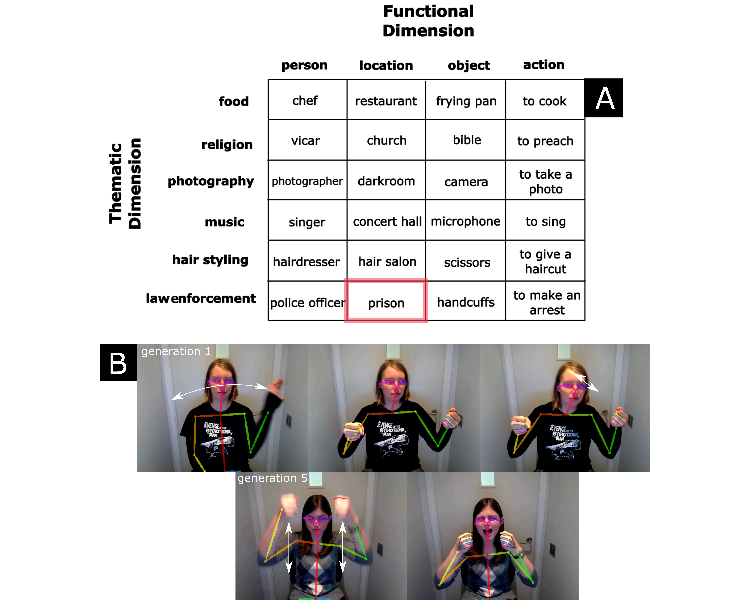
\includegraphics{GNet_WP_files/figure-latex/plotconcepts-1.pdf}
The thematic dimension captured concepts that were alike in what theme they could be grouped by; for example grouped by a ``religion'' theme. Gestures also had another \emph{functional} dimension to them, such that concepts consistently either referred to an action, person, location, or an object. The aforementioned dimensions thereby provide the axes for compressibility of the communicative tokens. After all, by combining 8 unique gestures one can pick out any referent (e.g., ``to make an arrest'') from the 36 token meaning space, one gesture marking the functional category (e.g., ``action'') and another gesture for the theme category (``justice'').\\
(Motamedi et al., 2019) showed with qualitative analysis that in beginning iterations of learning, gestures were particularly pantomimic in nature, whereby large-sized iconic enactments were the most common way of gesturally depicting the referents. However, novel ``grammatical'' gestures emerged over the generations, such that particular components were reused for different gestures. Particularly this reuse of components were cases of grammatical marking of the thematic and functional categories. Thus gesture communicative system seemed to become more compressible and systematic over the generations.\\
With meticulous hand-coding of the different referential components of each silent gesture, it could further be quantitatively tested whether there was indeed combinatorial structure emerging. Based on the the full sequence of the referential components, entropy was computed, which expresses the amount of information that is needed to compress a signal. When a lot of components recur at a higher chance, the system has a more simple structure (requires less information to be compressed), indicating combinatorial structure (e.g., Gibson et al., 2019). Dovetailing with the qualitative observations and other studies in this field (e.g., Verhoef et al., 2016), it was found that gesture-component' entropy decreased over the generations. Furthermore, the gesture's were coded for the amount of grammatical marking for the functional category, and this showed that such gestures occured more often at later generations. Finally, gesture duration - as a measure of communicative efficiency - was not reliably changing over the generations, which ran counter to predictions that more mature communication systems tend towards maximal efficiency.\\
These results obtained in the lab resonate with findings with homesign (e.g., Haviland, 2013) and emerging sign languages (Senghas, Kita, \& Özyürek, 2004). For example, it has been shown that in the expression of motion events first generation of Nicaraguan sign language performed more holistic presentations of path and manner, while in following generations manner path were segmented. Such segmentations affords novel combinatoriality and therefore increases generativity of a language; it increases the meaning space with fewer means similar to how participants studied by Motamedi et al. (2019) started to develop ways to express grammatical status of the referents.

\hypertarget{current-stage-1-study}{%
\subsection{Current stage-1 study}\label{current-stage-1-study}}

So far research on linguistic properties of manual or whole-body gesture have been based on human coding. Often this is theoretically well-justified because the kinematic signal as such - similar to acoustics in speech - does not specify the linguistic content of the signal (e.g., its semantic content). A community of language users is needed to decide on such meanings, with the human coder acting as the representatative. However, form-level systematicities can be revealing of linguistic structure, and the emergence of such combinatorial structure have been found in many different kind communicative signals, such as whistling signals controlled by a slider (Verhoef et al., 2016), drumming sequences (Ravignani, Delgado, \& Kirby, 2016), letter sequences (Cornish, Dale, Kirby, \& Christiansen, 2017), and a wide range of animal vocalizations (Engesser \& Townsend, 2019). A pressing challenge for applying a similar approach to silent gesture is how to quantify systemic changes from the continous and complex multi-articulatory movements. Specifically, while there have been progress in the current field in quantifying form similarity between silent gestures (e.g., Namboodiripad, Lenzen, Lepic, \& Verhoef, 2016; Sato et al., 2020), a still standing challenge is how to understand such kinematic events at higher levels of description, at the level of the communicative system as a whole.\\
Arguably, the study of communicative systems on the level of its interrelationships is crucial for detection of linguistic structure. To exemplify, a pantomime gesture that is repeated for many referents becomes saturated in meaning. An enlargement of a gesture trajectory to signal communicative salience, is maximally meaningful when such an enlargement is systematically repurposed in other gestures as well. Additionally, when studying language systems we are on the lookout for arbitrariness, which by its very logic requires for its detection a system-level view that approximates tokens' structural interrelationships while disregarding particular idiosyncracies of the tokens themselves.\\
In the current stage 1 research report we aim to address the broader challenge of relating complex multi-segmented kinematics with possible combinatorial structure emerging at the system level. To this end, we applied computer vision techniques (Cao et al., 2017b) to extract human movement traces from video data, and submitted these multidimensional time series to gesture network analysis (Pouw \& Dixon, 2019). Tios approach allows for a quantification of the interrelationships between communicative tokens (Sato et al., 2020; Verhoef et al., 2016). We further report which kinematic properties changed as the commmunicative system evolved, and how this relates to changes at the system level. In the final section of this report we overview our confirmatory stage 2 study where will adress predictions for experiment 2 and 3 of Motamedi et al. (2019). \pagebreak
\# Method
Figure 2 shows the general overview of the gesture network analysis procedure for this experiment. We will discuss each step in this procedure in the following sections. Then we will discuss our main network and kinematic outcome measures. Whereever possible we provide quantiative checks to motivate our particular choice of measurement.

\pagebreak

Figure 2. General method gesture network analysis
\includegraphics{GNet_WP_files/figure-latex/plotmainmethodfigure-1.pdf}
\small *Note Figure 2*. The general procedure is shown for the current gesture network analysis. A) shows the original experiment setup, where for each chain containing five generations a seedset was randomly selected of 24 seed gestures. These seed gestures were reproduced by the two participants in each generation during a director-matcher task. For our analysis we first performed video-based motion tracking with OpenPose (Cao et al., 2017a) to extract relevant movement traces (\(T_{i}\)) of the nose, the wrists and index fingers. For each gesture comparison within a gesture set, the time series were then submitted in C) to a Dynamic Time Warping (dtw) procedure where we computed for each body part a multivariate (i.e., x, y position traces) dtw normalized distance measure, which was repeated for all 5 body parts (nose, wrist left, wrist right, etc.) and summed, resulting in one overall distance measure (`D') between a gesture comparison. All D measures were saved into a matrix \(\textbf{\mbox{D}}\) containing all gesture comparisons \(D_{i,j}\) within the comparison set, resulting in a 24x24 distance matrix. The distance matrix can be visualized as a fully connected weigthed graph through multidimensional scaling, such that nodes indicate gesture utterances and the distance between gesture nodes the `D' measure, indicating dissimilarity. \normalsize 

\hypertarget{participant-design-procedure-of-the-original-study-experiment-1}{%
\subsubsection{Participant, design, \& procedure of the original study (experiment 1)}\label{participant-design-procedure-of-the-original-study-experiment-1}}

Here we will discuss as succinctly as possible the setup of the experiment which generated the data we reanalyzed. For a more detailed information we refer to Motamedi et al. (2019).\\
A seed gesture set was created with 48 pre-study participants who depicted 1 out of 24 concepts. Thus for each concept there were two seed gestures performed by unique pre-study participants. Given that pre-study participants only produced one gesture they were also unknown to the other concepts that comprised the meaning space.\\
For the main experiment (exp. 1) 50 right-handed, english-speaking, and non-signing, participants were recruited. They would be submitted to a particular chain (one of 5 chains) through which iterations of silent gesturing would cascade forward. Each iteration, or henceforth generation, consisted of two pairs of participants.\\
The participants at the start of each chain, during their training phase, were shown a subset of the seed gestures. Namely, 24 unique gestures were selected from the subset of 48 seed gesture-set, and were balanced per thematic and funcitonal dimension. These chain-specific seed gesture sets will be referred to as generation 0, which were followed by generations 1 through 5.\\
For each generation, during the training phase, silent gestures were presented in random order whereby participants needed to correctly identify the meaning of the gesture from the meaning space (24-item meaning-space), and then were given feedback about performance. Then participants were asked to copy the gesture in a self-timed manner. Participants trained with 36 items, with some gestures practiced twice.\\
During testing phase paired participants gesturally communicated a selected target meaning as a director to the other partner who needed to match the meaning. Feedback was provided about performance after each depiction. This director-matcher routine was repeated untill both participants gesturally depicted all 24 meanings.\\
After the testing phase a subsequent generation was initiated with a new pair of participants who were given a training set based on the gestures from one randomly selected participant from the parent pair. The child pair then went through the same procedure described above, and were the progenitors for the next generation.\\
The self-recordings of seed gestures, and the gestures participants produced in the testing phases, are the data that we use for our current analysis. This means that we have 50 x 24 = 1200 gestures belonging to generation 1-5, and 48 seed gesture videos.

\hypertarget{motion-tracking}{%
\subsubsection{Motion tracking}\label{motion-tracking}}

Motion tracking was performd on each video recoding with a maximum sampling rate of 30Hz (as circumscribed by 30 fps recording). To extract movement traces we used OpenPose (Cao et al., 2017a), which is a pretrained deep neural network approach for estimating human poses from video data (for a tutorial see Pouw \& Trujillo, 2019). We selected keypoints that were most likely to cover the gross variability in gestural utterances: positional x (horizontal) and y (vertical) movement traces belonging to left and right, index fingers, wrists, as well as the nose. For all position traces and its derivatives, we applied 1st order 30Hz low-pass butterworth filter to smooth out high frequency jitters having to do with sampling noise. We further z-normalized and mean-centered position traces for each video, so as to ensure that differences between subjects (e.g., body size) and within-subject differences in camera position at the start of the recording were inconsequential for our measurements.

\hypertarget{dynamic-time-warping-dtw}{%
\subsubsection{Dynamic Time Warping (DTW)}\label{dynamic-time-warping-dtw}}

DTW is a commmon signal processing algorithm to quantify similarity between temporally ordered signals (Giorgino, 2009; Mueen \& Keogh, 2016; Muller, 2007). The algorithm performs a matching procedure between two time series by maximally realligning (warping) nearest values in time while preserving order, and comparing their relative distances after this non-linear allignment procedure. The degree that the two timeseries need to be stretched and warped indicates how disimilar they are. This disimilarity is expressed with the DTW distance measure, with a higher distance score for more dissimlar timeseries and a lower score for more similar time series.\\
The time series in the current instance are multivariate, as we have a horizontal (x) and vertical (y) positional time-series data. However, DTW is easily generalizable to multivariate data, and can compute its distances in a multidimensional space per required, and this is then a multivariate dependent variant of DTW. We opt for a \emph{dependent} DTW procedure here as x an y positional data are part of a single position coordinate in space. Additionally, we have 6 of these 2-dimensional time series for each body keypoint. To compute a single distance measure between gestures, we therefore computed for each gesture comparison a multivariate dependent DTW Distance measure per keypoint, which was then summed for all keypoint comparisons to obtain a single \emph{Distance} (or simply `D') measure. The D measure thus reflects a general dissilimarity (higher D) or similarity (lower D) of the whole manual+head movement utterance versus another utterance.
We used R package `DTW' (Giorgino, 2009) to produce the multivariate distances per keypoint. The DTW distance measure was normalized for both time series' length, such that distances are expressed per unit time, rather than summed per unit time which would yield higher (and biased) distance estimates for longer timeseries (i.e., longer gesture videos). For further conceptual overview and methodological considerations of the current DTW procedure see (Pouw \& Dixon, 2019).

As a demonstration that our D measure reflects actual differences in kinematics, we computed for each individual in each chain the difference between a gesture seed and the gesture that the invidual produced to model it, for generation 1. These ``true pairs'' must be maximally similar (lower D) as the individual was thaught this gesture and will most closely reproduce this exact gesture (give or take some modifications). We contrast this with a false or random comparison of the same gesture in generation 1 with a gesture seed that was neither in the same functional nor thematic category. These false random pairs must be more dissimilar, and should produce higher DTW distances.
Figure 3 shows the distributions of the distances observed. DTW distance distributions were reliably different, \emph{t} (469.77) = 15.82, \emph{p} = \textless{} .001, Cohen's \emph{d} = 1.44, for the random pair, \emph{M} =2.78(\emph{SD} = 0.78), as compared to the random pair, \emph{M} = 3.84(\emph{SD} = 0.69).
Importantly, we also find that adding head movement trajectory to our D calculation significantly increases false-real pair discriminability as compared when we compute our D measure on only manual keypoints (left/right wrist and index fingers), change in Cohen's \emph{d} = 0.41, change D real vs.~false = 0.33, \emph{p} = \textless{} .001. Therefore we conclude, that in the current experiment the gesture utterances are also crucially defined by head movements as well. This is an interesting finding in and of itself, and demonstrates the co-articulatory nature of silent gestures.\\
Figure 3. Density distributions of D for true pairs and random pairs\\
\includegraphics{GNet_WP_files/figure-latex/plot_distributioncheck-1.pdf}
\emph{Note Figure 3}. The densitiy distributions of D are shown for the random versus real pairs. This D comparison is based on head-, wrists- and fingers movement comparisons. There is good discriminability between real versus falsely paired gestures, confirming that our approach is tracking gesture similarity well and we can proceed with the next methdological step.

\hypertarget{gesture-networks}{%
\subsubsection{Gesture networks}\label{gesture-networks}}

We constructed for each participant (nested in generation nested in chain), as well as each seed gesture set (seed set belonging to that chain), a distance matrix \(\textbf{\mbox{D}}\), containing the continous D comparisons for each gesture \(D_{i,j}\) produced by that participant. As such distance matrix \(\textbf{\mbox{D}}\) contains 24x24 cells. \(\textbf{\mbox{D}}\) is symmetric along its diagonal (as computing distance between gesture 1 and 2 is the same as computing distance btween gesture 2 and 1). The diagonal contains zeros for gesture comparisons that are identical (\(D_{i,j} = 0 | i=j\)). These characteristics make \(\textbf{\mbox{D}}\) a weighted symetric distance matrix.\\
From the distance matrices we can construct a visual representation of its topology by projecting the distance of gesture token on a 2d plane using multidimenstional scaling. These networks are fully connected graphs with distances between gesture nodes reflecting our D measure. This visual projection or network representation is an imperfect approximation of our multidimensional data contained by \(\textbf{\mbox{D}}\) and is only used as a visual aid in the current paper. Note though, that the uncompressed distance matrices are used to calculate the topological properties, i.e., interrelationships of communicative tokens. For short hand, we refer to these matrix properties as `network properties' as discuss below, as these measures are intuitively understood in network terms. Throughout we use R package `igraph' (Csárdi, 2019) for network visualisation and multidimensional scaling, as well as the calculation of network entropy.

\hypertarget{gesture-network-properties}{%
\subsection{Gesture Network Properties}\label{gesture-network-properties}}

\hypertarget{combinatorial-structure-network-entropy}{%
\subsubsection{Combinatorial structure: Network Entropy}\label{combinatorial-structure-network-entropy}}

The network entropy measure was produced with R package `igraph' and is almost identical to a classic Shannon entropy calculation, where \(Entropy\; H(X) = -\sum p(X)\log p(X)\). The only difference is that the entropy we computed on the weights of the networks' edges for each node relative to the shortest path to the other nodes (ie., connections; i.e., \(D_{i,j}\)), and then normalized by the number of connections.\\
Entropy is a measure that quantifies the compressibility of data structures, and has been used to gauge the combinatorial structure of communicative tokens in the field of language evolution (e.g., Verhoef et al., 2016; for theoretical grounding see Gibson et al., 2019). In the original experiment Motamedi computed entropy from the gesture content codings, whereby it is assessed whether particular gesture content was recurring. In our case entropy quantifies the degree to which similar length edges are less diverse (come from more peaked probability distributions), and if so, this means that the communicative tokens relate in more structural ways to each other.\\
To explain entropy with some simple (but contrived) examples: if we have a network, where the chance of having an edge length of D = x is 1, then the network connections are fully compressible and we yield an entropy of 0 (\(Entropy = -1 * 1 * log(1) = 0\)). Now, if in fact there are different edge lengths (increasing the complexity of our network) such that we have a 0.5 chance that \(D = x\) and 0.5 chance that \(D = y\), then entropy goes up, \(Entropy = -1 * 0.5 * log(0.5) = 0.34\). Remember, that the log of a fraction becomes a negative number, that is why the result is multiplied by -1 at the start of the formula. Note further that when the system is so diverse that there is a almost zero chance that any connection is recurring, entropy will aproach infinity (the system is incompressible). To generalize this for our case, when entropy goes up, it means that communicative tokens interrelate in a more random way (i.e., the system is more complex; i.e., has less combinatorial structure), while if entropy goes down, it means that communicative tokens interrelate more structurally.

\hypertarget{clustering}{%
\subsubsection{Clustering}\label{clustering}}

A further interesting property of the communicative tokens' interrelationships is the degree to which they cluster or differientate from each other. Clustering would indicate that there are multiple gestures that have similar features, which may indicate lack of differientability and increases in associability. Indeed, we might expect that communicative tokens within a theme are likely to be ambiguous at beginning generations (e.g., the ambiguous reuse of the handcuffing gesture for `to make an arrest' and `police officer') and such gestures would cluster with edge weigths of low D.\\
For the clustering measure we use a technique from Topological Data analysis (e.g., Sizemore, Phillips-Cremins, Ghrist, \& Bassett, 2018) called persistent homology analysis (Bendich, Marron, Miller, Pieloch, \& Skwerer, 2016; Otter, Porter, Tillmann, Grindrod, \& Harrington, 2017), which can assess how stable (i.e., persistent) network components are through a continous quantification (for an accessible introduction to persistent homology see e.g., \href{https://www.youtube.com/watch?v=E7d7LHb6PLc}{youtube link}).\\
Consider that the distance matrices contain coordinates for each gesture in a multidimensional space relative to all other gestures. What persistent homology does is iteratively ramp up a threshold that determines when nodes (i.e., gestures) get connected by an edge connection (see figure 4). As shown in Figure 3, the treshold can be seen as a radius around each node that expands (in our case in a multidimensional space). Whenever the sphere touches another node's sphere, a graph is updated such that these nodes get connected with an edge connection. At the beginning of this iteration process, there are only components with no connections. But as the spheres expand, connections are made. When connections are made new components get born and components will die as they are overtaken. Through this process it can quantified for `how long' certain components (called 0-cycles) persist during the expansion of the radius (there are also other structures such as loops or 1-cycles that can be trackced, but we will not use this here). If a structure of connected nodes remains intact over more iterations of expansion, without any new connections being added to this structure, then it means that this structure is stable (i.e., persistent). Such persistent components or clusters survive for longer time during these expansions as these structures are born fast (the structure's members are in close proximity) and die late (as the structure is far removed from other nodes or structures) during the iterative expansion. The average persistence of the components (time of death minus time of birth) thus is a measure of clustering.\\
To compute cluster persistence we used R-package `TDAstats' (Wadhwa et al., 2019). We averaged persistence for the statistically significant components only, by using TDAstats bootstrapping method (at chance level of 0.975). The selection of statistically reliable components was applied as many components that are detected during the iteration process are of very short persistence and reflect noise/chance level occurences of components. We computed the average persistence of components (0-cycles) for each distance matrix (i.e., each individual's gesture network).

Figure 4. Network property example\\
\includegraphics{GNet_WP_files/figure-latex/networkprop_plot-1.pdf}
\small *Note Figure 4.* A visual example is shown of the Topological Data Analysis procedure called `persistent homology'. Each (gesture) vertex has a certain distance to all vertices in the ensemble, and persistent homology analysis (PH) assesses the stability of components in this spatial organization. PH does this by increasing a spatial treshold (the radius) at which nodes get connected, as indicated here by red growing radii around each node. Whenever these spheres overlap, a graph gets updated and vertices get connected (and a new component is born). When there are stable components, this means that spheres have a relatively longer time to grow before the component's expanding sphere touches another component's expanding sphere.\normalsize    
Persistent homology is beneficial for mutidimensional data structures like the weighted fully connected distance matrices we are working with. This is because it allows for a continuous quantification of cluster stability at multiple scales (clusters of clusters), which is to be constrasted with a binary assignment of nodes to a particular cluster. Since Topological Data Analysis is relatively new analysis toolkit in cognitive science (Lum et al., 2013), we also made a comparison with another classic clustering measure as produced by a more well-known hierarchical clustering analysis algorithm (using an ``average'' method). We computed for each matrix the ``agglomerative clustering coefficient'' with R package `cluster', whereby a low clustering coefficient indicates more clustering in the data while a larger value indicates less clustering. We indeed find (see Figure 5) that when cluster persistence is high that the clustering coefficient is structurally lower, indicating that both measures are converging on their estimate of `clusteriness' of the data, \emph{r} = -0.39, \emph{p} = \textless{} .001. Hereonafter, we will only report the cluster persistence as a measure of clusteriness.

Figure 5. Cluster measure comparison\\
\includegraphics{GNet_WP_files/figure-latex/network_manip_check2-1.pdf}

\emph{Note Figure 5.} Higher cluster persistence is related to a lower agglomerative cluster coefficient, indicating that both measures are tracking some clustering property in the matrices.

\hypertarget{kinematic-properties}{%
\subsection{Kinematic Properties}\label{kinematic-properties}}

Gesture network analysis aims to target structural properties existing on the system level, whereby the \emph{interrelationships} of communicative tokens are studied rather than the content of those tokens. However, it is equally insightful to understand what specific changes occur in the kinematics of the gestures. Such specific changes might predict particular changes on the system level.\\
We first selected some potential measures representative for kinematic quality of the movements in terms segmentation (sg), salience (sl) and temporality (t), namely submovements (sg), smoothness (sg), gesture space (sl), rhythm (t), and rhythmiticity (t). See Figure 6 for two example time series from which most measures can be computed. All measures were computed for each keypoint' time series seperately and then averaged so as to get a grand score for the multimodal utterance as a whole. We eventually selected three measures tracking gesture intermittency (smoothness score), gesture salience (gesture space), gesture's temporality (rhythmiticity). Correlations and distributions are shown in Figure 7.

Figure 6. Overview kinematic measures
\includegraphics{GNet_WP_files/figure-latex/plotjerk-1.pdf}
\emph{Note Figure 6}. \small Two timeseries (belonging to two unique trials) are shown for right-hand wrist speed. From these time series, as well as the time series for other body parts, we computed measures tracking segmentation, namely, submovements (number of observed peaks in red) and smoothness (log dimensionless jerk). We further computed measures concerning temporality, namely the average time between submovements, i.e., rhythm in Hertz. We also computed rhythmicity, which is the standard deviation of the rhythm. Gesture space was calculated from the x,y position traces and is not shown here. \normalsize

We first computed a submovement measurement similarly implemented by Trujillo, Vaitonyte, Simanova, \& Özyürek (2019). Submovements are computed with a basic peak finding function which identifies and counts maxima peaks in the movement speed time series. We set the minimum interpeak distance at 8 frames, and minimum height = -1 (z-scaled; 1 std.), minimum rise = 0.1 (z-scaled). We logtransformed the submovement measure due to a skewed distribution.

\hypertarget{gesture-segmentation}{%
\subsubsection{Gesture segmentation}\label{gesture-segmentation}}

A property of the submovement measure is that it discretizes continuous information and uses arbitrary thresholds for what counts as a submovement, thereby risking information loss about subtle intermittencies in the movement. To have a more continuous measure of smoothness/intermittency of the movement we computed a dimensionless jerk measure (Hogan \& Sternad, 2009). This measure is dimensionless in the sense that it is scaled by the maximum observed movement speed and duration of the movement. Dimensionless jerk is computed using the following formula \(\int_{t2}^{t1} x''' (t)^{2}dt)* \frac{D^{3}}{max(v^{2})}\), where \(x'''\) is jerk, which is squared and integrated over time and multiplied by duration \(D\) cubed over the maximum squared velocity \(max(v^{2})\). As figure 6 shows, this measure correlates very highly with submovements, thus we chose to only use smoothness for further analysis. We logtransformed our smoothness measure due to a skewed distribution. Note that a \emph{higher} smoothness score indicates more intermittent (less smooth) movement.

\hypertarget{gesture-salience}{%
\subsubsection{Gesture salience}\label{gesture-salience}}

As a measure for gesture salience or reduction, we computed a gesture space measure. This was determined by extracting the maximum vertical amplitude of a keypoint multiplied by the maximum horizontal amplitude, i.e., the area in pixels that has been maximally covered by the movement.

\pagebreak

Figure 7. Correlations and distributions for kinematic measures per trial
\includegraphics{GNet_WP_files/figure-latex/summ_kin-1.pdf}
\emph{Note Figure 7}. Left upper panel, correlations and distributions are shown for smoothness and submovement. Given their high correlation we will use smoothness score for our final analysis. Other correlations are shown for the selected measures, rhythmiticy, gesture space and smoothness.

\hypertarget{gesture-temporality}{%
\subsubsection{Gesture temporality}\label{gesture-temporality}}

From the submovement measure we computed the average interval between each submovement (in Hz), which is a measure of rhythm tempo. This measure was, as expected, highly correlated with smoothness score as when more segmented movements are performed in the same time window, tempo goes up, \emph{r} = 0.8, \emph{p} = \textless{} .001, which led us to drop this measure for our analysis. Another temporal measure that is more orthogonal to smoothness and gesture space and which we will therefore include captures the stability of the rhythm, i.e., the rhythmicity of the movements. This measure is simply the standard deviation of the of the interval between submovements (given in Hz). Note, this measure cannot be calculated when there are less than 3 submovements (i.e., when there no intervals to detect the rhythmicity of).\pagebreak

\hypertarget{results}{%
\section{Results}\label{results}}

We will first report findings on how the communicative tokens interrelationships changed over the generations, as indicated by our network measures. Subequently, we will assess whether changes occurred between particular tokens, namely the function vs.~theme grouping. Finally, we will report on whether structural kinematic changes occured over the generations, and how such changes were predictive for changes on the network level.

\hypertarget{network-changes-over-generations}{%
\subsection{Network changes over generations}\label{network-changes-over-generations}}

Figure 8 shows that for the gesture networks, that entropy was generally decreasing as a function of generation, indicating a lower complexity of gesture interrelations as the system matures. Furthermore we obtain that clustering persistence was less pronounced at later generations.

\pagebreak

Figure 8. Changes in networks measures over generations within chains

\begin{figure}

{\centering \includegraphics{GNet_WP_files/figure-latex/plotresults-1} 

}

\caption{ }\label{fig:plotresults}
\end{figure}

\emph{Note Figure 8.} \small For each chain the changes over generations in entropy and cluster persistence is shown, with generation 0 indicating the seed gesture set. For each generation \textgreater{} 0 there are two data points as there are two participants in each generation. To example data points (red, and blue) are shown with their corresponding red and blue network representation (lower panel). In general cluster persistence decreased, indicating less differientability between tokens. This may be seen in example A where there are relatively large cavities between tokens, while in example B the token organization is more homegenously tesselated. Indeed, entropy tends to decline over the generations, indicating that relationships between tokens became less diverse, possibly indicating some combinatorial structure. \normalsize

We tested these trends seperately for each network property with mixed linear regression models, with chain as random intercept (random slopes did not converge for these models) and generation as independent predictor (0-5 generations, with generation 0 being the seed gesture network).\\
Generation was a reliable predictor for entropy as compared to a basemodel predicting the overall mean, chi-squared change (1) = 4.75, \emph{p} = 0.03, model \emph{R}-squared = 0.08. Model estimates showed that with increased generation the entropy decreased, \emph{b} estimate = -0.0006, \emph{t} ( 48.00 ) = -2.19, \emph{p} = 0.03).\\
Cluster presistence however was predicted by generation as compared to a basemodel, chi-squared change (1) = 14.61, \emph{p} \textless.001, model R-squared = 0.24. Model estimates showed that with increased generation the cluster persistence decreased, \emph{b} estimate = -0.09, \emph{t} (48.00) = -4.02, \emph{p} \textless{} .001).

\hypertarget{changes-within-them-versus-changes-within-function}{%
\subsection{Changes within them versus changes within function}\label{changes-within-them-versus-changes-within-function}}

We can further localize where combinatorial structure is most likely to increase (i.e., decrease in entropy) by subsetting the communicative tokens based on theme and function groupings. Thus for each participant we computed for gesture-networks grouped by e.g., action and computed network entropy. This was done for all categories and averaged to yield entropy within function categories. This was also done for thematic categories. See figure 9 for the main results of these subset networks.

\pagebreak

Figure 9. Change in entropy in theme-level networks versus function-grouped networks
\includegraphics{GNet_WP_files/figure-latex/funthemeentropy-1.pdf}
\emph{Note Figure 9}.\small On the left panel average network entropy for the function-grouped gestures are plotted over the generations with red line showing the trend averaged over chain (other-colored lines). On the right panel this is shown for the gestures grouped by theme category. It can be seen that only the function-grouped gesture networks showed increased combinatorial structure over the generations. \normalsize

Interestingly, we find that only functionally grouped tokens were minimizing entropy over the generations. Including generations for predicting function-level network entropy increased predictablilty as compared to a base model (random intercept chain, random slopes did not converge), chi-squared change (1) = 8.53, \emph{p} = 0.00, model \emph{R}-squared = 0.14, with generation relating to lower entropy \emph{b} estimate = -0.0013, \emph{t} ( 48.00 ) = -3.00, \emph{p} = 0.00).\\
There was however no reliable decrease in entropy for the theme-level networks, chi-squared change (1) = 0.18, \emph{p} = 0.67, model \emph{R}-squared = 0.00, with generation not reliably relating to entropy \emph{b} estimate = 0.0005, \emph{t} ( 48.00 ) = 0.41, \emph{p} = 0.68).

\hypertarget{kinematic-features}{%
\subsection{Kinematic features}\label{kinematic-features}}

We also performed mixed regression analysis for assessing potential kinematic changes as a function of generation, with random intercept for objects nested within chains (random slopes did not converge). See figure 10 for main results.

Figure 10. Change in kinematic properties over generations\\

\begin{figure}

{\centering \includegraphics{GNet_WP_files/figure-latex/kinematicresults-1} 

}

\caption{ }\label{fig:kinematicresults}
\end{figure}

\emph{Note Figure 10}. \small Generation trends per chain are shown for smoothness, rhythmicity and gesture space. Each observation indicates a communicative token, and these are spatially organized per their density distribution. We can see that over the generations are more smooth/less segmented movements (lower smoothness score), with a more stable rhythm (lower rhythmicity score), and more minimized movements (smaller gesture space). Note, that rhythmicity has lower data points as often the movement did not consist of more than 2 submovements. Thus rhythmicity indicates, that when there is a multisegmented movement, then such movements were more rhythmic. \normalsize

Generations reliably predicted smoothness of the movements relative to a basemodel, chi-squared change (1) = 76.66, \emph{p} \textless.001, model \emph{R}-squared = 0.06, with generation predicting lower smoothness score, \emph{b} estimate = -0.2263, \emph{t} ( 1,135.00 ) = -8.90, \emph{p} \textless{} .001).
We also observe higher rhytmicity as a function of generations, chi-squared change (1) = 24.12, \emph{p} \textless.001, model \emph{R}-squared = 0.05, indicating more stable rhythmic movements at later generations, \emph{b} estimate = -0.0693, \emph{t} ( 332.00 ) = -4.97, \emph{p} \textless{} .001).\\
Finally, over the generations gesture space decreased, chi-squared change (1) = 24.45, \emph{p} \textless.001, model \emph{R}-squared = 0.00. Model estimated gesture space was less for later generations, \emph{b} estimate = -2.2100, \emph{t} ( 1,174.00 ) = -4.97, \emph{p} \textless{} .001).\\
In conclusion, our kinematic results show all the hallmarks of communicative efficiency. Namely, gestures were on average small, more rhythmic, and less intermittent as the communicative system matured.

\hypertarget{kinematic-features-and-network-properties}{%
\subsection{Kinematic features and network properties}\label{kinematic-features-and-network-properties}}

Figure 11 contains the correlations of the relationships of kinematic properties (average per participant) and the network measures cluster persistence and entropy. Network entropy goes down as the average gesture space decreases, the movement becomes more less intermittent (lower smoothness score). This also comes at a tradeoff, such that this simplification of kinematics, also reduces differientiability of communicative tokens as there is less stable clustering when gesture become smaller, more rhythmic, and smoother (less intermittent). Thus on the kinematic level there seems to be a general decrease of complexity which is further reflected on the level of the system as a whole as utterances become less \emph{kinematically} differientable (less clustering) and more structured in their relations (lower entropy).

\pagebreak

Figure 11. Relation between kinematic properties and network measures
\includegraphics{GNet_WP_files/figure-latex/test_network_kinematics-1.pdf}
\emph{Note Figure 10}. \small Correlations are shown for each kinematic property averaged over all utterances and the concomittant network measure result. It can be seen that stable rhythms (lower rhythmicity score), less intermittency (lower smoothness score), and smaller gesture space (lower gesture space score), relates to lower entropy and lower cluster persistence. This indicates that complexity in movement is cashed out in terms of combinatorial structure on the network level and lower differentiability in terms of cluster instability. \normalsize

\pagebreak

\hypertarget{discussion}{%
\section{Discussion}\label{discussion}}

Pattee argued that one of the great problems in science is to characterize how symbolic discrete strings (e.g., DNA) emerge from biological, continuous, and dynamical processes (Pattee \& Rączaszek-Leonardi, 2012). In the current research we address a comparable problem, whereby we assessed how we can detect from continuous multi-articulatory kinematics of silent gestures, possible systematic changes reflective of a linguistically maturing communcaton system. We applied computer vision techniques to extract kinematics from videodata, and then applied an analysis procedure to detect structural relations between multimodal utterances (Pouw \& Dixon, 2019).
Our findings indicated that the interrelationships between communicative tokens had higher combinatorial structure at later generations, conceptually replicating results that were based on human coding of the gesture's content (Motamedi et al., 2019). We extend these findings by showing that tokens were less stably differientable on the form level as tokens have lower cluster persistence over the generations. Interestingly, especially the functionally grouped gestures showed increase in combinatorial structure, rather than the arguably more concrete thematic grouping. While in the original study no increase in efficiency was found based on measuring gesture duration, we did detect signs of communicative efficiency for gesture kinematics. Namely, over the generations, gestures became less segmented (more smooth), more rhythmic (if comprised of more than 3 submovements), and decreased in size. Finally, we show that this decrease in kinematic complexity on the token level, predicts system-level changes of decreased entropy and decrease is clustering.\\
A decrease in cluster persistence over generations here is likely to reflect an increase in homegenous interrelationships between the communicative tokens, which as originally reported often showed iconic gestures at early stages in the iterations that were sometimes ambiguous in the theme category, and maximally differientated from the other-themed gestures. For example, ``arrest'' and ``police officer'' could both contain a gesture that enacts the appliance of hand cuffs. When such gestures are disuambiguated this will result in increased distances among the gestures within this category on the network level, i.e., will lead to contributing to less clustering. Yet, while clusters became more instable over the generations, the diversity of the interrelationships of the communicative tokens decreased (i.e., entropy decresed). This suggests that there is a more consistent and thus homogenous, way in which the communicative system is organized. That this increase in consistency is indeed a systematic process is further supported the detection of entropy decrease over the generations for communicative tokens that are grouped on a more abstract functional level (e.g., agent, action, location), as opposed to the thematic level (e.g., justice, cooking). Thus structure is particular emerging among tokens that reflect a more abstract property such as reference classes.\\
The kinematic findings suggest that the manual utterances simplify, in the way of reducing in size, in the reduction of submovements and the increase in the rhythmicity. Interestingly, this is precisely what one finds for novice learners of ASL. ASL learners have been found to spatially reduce their signs as they become more fluent (Lupton \& Zelaznik, 1990; Wilbur, 1990). Moreover, a reduction in duration between the compounds of the signs have been observed during learning progression, where multicomponent component signs are increasingly performed as a single sign. In the present paradigm, there is also likely an evolution of pronounciation in this way, such that multimodal utterances acquire stable functional organizations across generations. Suboptimal organization of sub-movements will be filtered out as it were over the generations, and the temporally extended movement sequence becomes likely more coordinated whereby degrees of freedom are reduced by functioning as a single multimodal coordinative structure (Bernstein, 1967; Kelso, Tuller, \& Harris, 1983; Kelso \& Tuller, 1984), affecting for example gesture's rhytmicicty and smoothness. That head movements improved differientation of real vs.~falsely paired gestures in our analysis, further emphasize that there multiple articulators coordinate in the production of meaning. This finding resonates with the known grammatic, phonetic, and prosodic functions that head movements have in sign languages such as ASL (Tyrone \& Mauk, 2016).\\
It is tempting to ask then whether the current entropy decrease on the system level is a function of perceptual-motor development of the utterances or rather of some kind of optimal segmentation of the utterance as originally observed when independent raters judge the types of meaningful segments (Motamedi et al., 2019). However, these results are not mutually exclusive we think. It is rather likely that a general tendency for optimal organization on the level of perception-action coordination also participates in the seeking of optimal ways of segmenting a communicative message. Perception-action constraints \emph{are} then are linguistic constraints.\\
However, an important caveat to the current analysis is that kinematic analyses have limits in general, and the current analysis has specific limits with regards to temporal ordering. In general, it is the case kinematic analysis cannot say anything about the semiotic content that might evolve, and this is especially the case with incereasing `drifts towards the arbitrary' (Tomasello, 2008). Although such drift might be detected via our network analysis, the current analyses do no precluded the necessity of human coders as representatives of the language community. Thus the current analysis are only helpful to scale up automatic signal-based approaches to the study of gestural communication, not to replace analyses that require human coders.\\
There is further a specific shortcoming to the current analysis, which centers on the particular properties of the dynamic time warping algorithm. Namely, if we appreciate that combinatorics increases as a communicative system matures, the holistic gestures become segemented and the order of presentaiton of such segements might be (meaningfully) varied. However, the DTW algorithm is sensitive to ordering and would judge two gestures containing identical segments in different orders as very different, while for a human coder the similarity is transparent. Thus our analysis may at times judge dissimilarity due to changes in order, rather than changes in kinematics as such. There are ways to circumvent this, using a different kinematic time series analysis as we discuss in Pouw \& Dixon (2019), but such analysis that goes beyond the current approach. In sum, the current approach is imperfect, but we believe given that it is fully reproducable and automatable approach it promises to help scale up the evolution of language in the manual and whole-body modality.

\hypertarget{pre-registration}{%
\section{Pre-registration}\label{pre-registration}}

TO-DO - after our meeting I will finish this section

We hypothesize that xx

\hypertarget{experiment-2}{%
\subsection{Experiment 2}\label{experiment-2}}

\hypertarget{experiment-3}{%
\subsection{Experiment 3}\label{experiment-3}}

\hypertarget{references}{%
\section{References}\label{references}}

\begingroup
\setlength{\parindent}{-0.5in}
\setlength{\leftskip}{0.5in}

\hypertarget{refs}{}
\begin{cslreferences}
\leavevmode\hypertarget{ref-aronoffRootsLinguisticOrganization2008}{}%
Aronoff, M., Meir, I., Padden, C. A., \& Sandler, W. (2008). The roots of linguistic organization in a new language. \emph{Interaction Studies}, \emph{9}(1), 133--153. doi:\href{https://doi.org/10.1075/is.9.1.10aro}{10.1075/is.9.1.10aro}

\leavevmode\hypertarget{ref-bausWhenDoesIconicity2013}{}%
Baus, C., Carreiras, M., \& Emmorey, K. (2013). When does Iconicity in Sign Language Matter? \emph{Language and Cognitive Processes}, \emph{28}(3), 261--271. doi:\href{https://doi.org/10.1080/01690965.2011.620374}{10.1080/01690965.2011.620374}

\leavevmode\hypertarget{ref-bavelasGesturingTelephoneIndependent2008}{}%
Bavelas, J., Gerwing, J., Sutton, C., \& Prevost, D. (2008). Gesturing on the telephone: Independent effects of dialogue and visibility. \emph{Journal of Memory and Language}, \emph{58}(2), 495--520. doi:\href{https://doi.org/10.1016/j.jml.2007.02.004}{10.1016/j.jml.2007.02.004}

\leavevmode\hypertarget{ref-bendichPersistentHomologyAnalysis2016}{}%
Bendich, P., Marron, J. S., Miller, E., Pieloch, A., \& Skwerer, S. (2016). Persistent Homology Analysis of Brain Artery Trees. \emph{The Annals of Applied Statistics}, \emph{10}(1), 198--218. doi:\href{https://doi.org/10.1214/15-AOAS886}{10.1214/15-AOAS886}

\leavevmode\hypertarget{ref-bernsteinCoordinationRegulationsMovements1967}{}%
Bernstein, N. (1967). \emph{The Co-ordination and Regulations of Movements} ({[}1st English ed.{]} edition.). Pergamon Press.

\leavevmode\hypertarget{ref-bickertonAdamTongue2009}{}%
Bickerton, D. (2009). \emph{Adam's Tongue}. New York: Hill \& Wang.

\leavevmode\hypertarget{ref-cangelosiSimulatingEvolutionLanguage2002}{}%
Cangelosi, A., \& Parisi, D. (Eds.). (2002). \emph{Simulating the Evolution of Language}. London: Springer-Verlag. doi:\href{https://doi.org/10.1007/978-1-4471-0663-0}{10.1007/978-1-4471-0663-0}

\leavevmode\hypertarget{ref-caoRealtimeMultiPerson2D2017}{}%
Cao, Z., Simon, T., Wei, S.-E., \& Sheikh, Y. (2017a). Realtime Multi-Person 2D Pose Estimation Using Part Affinity Fields. In (pp. 7291--7299). Presented at the Proceedings of the IEEE Conference on Computer Vision and Pattern Recognition. Retrieved from \url{http://openaccess.thecvf.com/content_cvpr_2017/html/Cao_Realtime_Multi-Person_2D_CVPR_2017_paper.html}

\leavevmode\hypertarget{ref-caoRealtimeMultiperson2D2017}{}%
Cao, Z., Simon, T., Wei, S.-E., \& Sheikh, Y. (2017b). Realtime Multi-person 2D Pose Estimation Using Part Affinity Fields. In \emph{2017 IEEE Conference on Computer Vision and Pattern Recognition (CVPR)} (pp. 1302--1310). Honolulu, HI: IEEE. doi:\href{https://doi.org/10.1109/CVPR.2017.143}{10.1109/CVPR.2017.143}

\leavevmode\hypertarget{ref-christiansenNoworNeverBottleneckFundamental2016}{}%
Christiansen, M. H., \& Chater, N. (2016). The Now-or-Never bottleneck: A fundamental constraint on language. \emph{Behavioral and Brain Sciences}, \emph{39}. doi:\href{https://doi.org/10.1017/S0140525X1500031X}{10.1017/S0140525X1500031X}

\leavevmode\hypertarget{ref-claidiereCulturalEvolutionSystematically2014}{}%
Claidière, N., Smith, K., Kirby, S., \& Fagot, J. (2014). Cultural evolution of systematically structured behaviour in a non-human primate. \emph{Proceedings of the Royal Society B: Biological Sciences}, \emph{281}(1797), 20141541. doi:\href{https://doi.org/10.1098/rspb.2014.1541}{10.1098/rspb.2014.1541}

\leavevmode\hypertarget{ref-corballisHandMouthOrigins2002}{}%
Corballis, M. C. (2002). \emph{From hand to mouth: The origins of language}. Princeton, NJ.: Princeton University Press.

\leavevmode\hypertarget{ref-cornishSequenceMemoryConstraints2017}{}%
Cornish, H., Dale, R., Kirby, S., \& Christiansen, M. H. (2017). Sequence Memory Constraints Give Rise to Language-Like Structure through Iterated Learning. \emph{PLOS ONE}, \emph{12}(1), e0168532. doi:\href{https://doi.org/10.1371/journal.pone.0168532}{10.1371/journal.pone.0168532}

\leavevmode\hypertarget{ref-csardiPackageIgraphNetwork2019}{}%
Csárdi, G. (2019). Package 'igraph' Network Analysis and Visualization (Version 1.2.4.1). Retrieved from \url{http://bioconductor.statistik.tu-dortmund.de/cran/web/packages/igraph/igraph.pdf}

\leavevmode\hypertarget{ref-deutscherUnfoldingLanguageEvolutionary2005}{}%
Deutscher, G. (2005). \emph{The Unfolding of Language: An Evolutionary of Mankind's Greatest Invention}. New York: Metropolitan Books.

\leavevmode\hypertarget{ref-dingemanseArbitrarinessIconicitySystematicity2015b}{}%
Dingemanse, M., Blasi, D. E., Lupyan, G., Christiansen, M. H., \& Monaghan, P. (2015). Arbitrariness, Iconicity, and Systematicity in Language. \emph{Trends in Cognitive Sciences}, \emph{19}(10), 603--615. doi:\href{https://doi.org/10.1016/j.tics.2015.07.013}{10.1016/j.tics.2015.07.013}

\leavevmode\hypertarget{ref-dingemanseUniversalPrinciplesRepair2015}{}%
Dingemanse, M., Roberts, S. G., Baranova, J., Blythe, J., Drew, P., Floyd, S., \ldots{} Enfield, N. J. (2015). Universal Principles in the Repair of Communication Problems. \emph{PLoS ONE}, \emph{10}(9). doi:\href{https://doi.org/10.1371/journal.pone.0136100}{10.1371/journal.pone.0136100}

\leavevmode\hypertarget{ref-donaldOriginsModernMind1991}{}%
Donald, M. (1991). \emph{Origins of the modern mind: Three stages in the evolution of culture and cognition}. Boston: Harvard University Press.

\leavevmode\hypertarget{ref-dunbarHumanEvolutionOur2016}{}%
Dunbar, R. (2016). \emph{Human Evolution: Our Brains and Behavior}. Oxford: Oxford University Press.

\leavevmode\hypertarget{ref-engesserCombinatorialityVocalSystems2019}{}%
Engesser, S., \& Townsend, S. W. (2019). Combinatoriality in the vocal systems of nonhuman animals. \emph{WIREs Cognitive Science}, \emph{10}(4), e1493. doi:\href{https://doi.org/10.1002/wcs.1493}{10.1002/wcs.1493}

\leavevmode\hypertarget{ref-fayInteractiveEvolutionHuman2010}{}%
Fay, N., Garrod, S., Roberts, L., \& Swoboda, N. (2010). The interactive evolution of human communication systems. \emph{Cognitive Science}, \emph{34}(3), 351--386. doi:\href{https://doi.org/10.1111/j.1551-6709.2009.01090.x}{10.1111/j.1551-6709.2009.01090.x}

\leavevmode\hypertarget{ref-fitchMonkeyVocalTracts2016}{}%
Fitch, W. T., Boer, B. de, Mathur, N., \& Ghazanfar, A. A. (2016). Monkey vocal tracts are speech-ready. \emph{Science Advances}, \emph{2}(12), e1600723. doi:\href{https://doi.org/10.1126/sciadv.1600723}{10.1126/sciadv.1600723}

\leavevmode\hypertarget{ref-frohlichMustAllSignals2020}{}%
Fröhlich, M., \& van Schaik, C. P. (2020). Must all signals be evolved? A proposal for a new classification of communicative acts. \emph{WIREs Cognitive Science}. doi:\href{https://doi.org/10.1002/wcs.1527}{10.1002/wcs.1527}

\leavevmode\hypertarget{ref-garrodFoundationsRepresentationWhere2007}{}%
Garrod, S., Fay, N., Lee, J., Oberlander, J., \& Macleod, T. (2007). Foundations of representation: Where might graphical symbol systems come from? \emph{Cognitive Science}, \emph{31}(6), 961--987. doi:\href{https://doi.org/10.1080/03640210701703659}{10.1080/03640210701703659}

\leavevmode\hypertarget{ref-gardenforsDemonstrationPantomimeEvolution2017}{}%
Gärdenfors, P. (2017). Demonstration and Pantomime in the Evolution of Teaching. \emph{Frontiers in Psychology}, \emph{8}. doi:\href{https://doi.org/10.3389/fpsyg.2017.00415}{10.3389/fpsyg.2017.00415}

\leavevmode\hypertarget{ref-gerwingLinguisticInfluencesGesture2004}{}%
Gerwing, J., \& Bavelas, J. (2004). Linguistic influences on gesture's form. \emph{Gesture}, \emph{4}(2), 157--195. doi:\href{https://doi.org/10.1075/gest.4.2.04ger}{10.1075/gest.4.2.04ger}

\leavevmode\hypertarget{ref-ghazanfarEvolutionHumanVocal2008}{}%
Ghazanfar, A. A., \& Rendall, D. (2008). Evolution of human vocal production. \emph{Current Biology: CB}, \emph{18}(11), R457--460. doi:\href{https://doi.org/10.1016/j.cub.2008.03.030}{10.1016/j.cub.2008.03.030}

\leavevmode\hypertarget{ref-gibsonHowEfficiencyShapes2019}{}%
Gibson, E., Futrell, R., Piantadosi, S. P., Dautriche, I., Mahowald, K., Bergen, L., \& Levy, R. (2019). How Efficiency Shapes Human Language. \emph{Trends in Cognitive Sciences}, \emph{23}(5), 389--407. doi:\href{https://doi.org/10.1016/j.tics.2019.02.003}{10.1016/j.tics.2019.02.003}

\leavevmode\hypertarget{ref-giorginoComputingVisualizingDynamic2009}{}%
Giorgino, T. (2009). Computing and Visualizing Dynamic Time Warping Alignments in \emph{R} : The \textbf{Dtw} Package. \emph{Journal of Statistical Software}, \emph{31}(7). doi:\href{https://doi.org/10.18637/jss.v031.i07}{10.18637/jss.v031.i07}

\leavevmode\hypertarget{ref-goldin-meadowNaturalOrderEvents2008}{}%
Goldin-Meadow, S., So, W. C., Özyürek, A., \& Mylander, C. (2008). The natural order of events: How speakers of different languages represent events nonverbally. \emph{Proceedings of the National Academy of Sciences}, \emph{105}(27), 9163--9168. doi:\href{https://doi.org/10.1073/pnas.0710060105}{10.1073/pnas.0710060105}

\leavevmode\hypertarget{ref-havilandEmergingGrammarNouns2013}{}%
Haviland, J. B. (2013). The emerging grammar of nouns in a first generation sign language: Specification, iconicity, and syntax. \emph{Gesture}, \emph{13}(3), 309--353. doi:\href{https://doi.org/10.1075/gest.13.3.04hav}{10.1075/gest.13.3.04hav}

\leavevmode\hypertarget{ref-hoganSensitivitySmoothnessMeasures2009}{}%
Hogan, N., \& Sternad, D. (2009). Sensitivity of Smoothness Measures to Movement Duration, Amplitude and Arrests. \emph{Journal of Motor Behavior}, \emph{41}(6), 529--534. doi:\href{https://doi.org/10.3200/35-09-004-RC}{10.3200/35-09-004-RC}

\leavevmode\hypertarget{ref-hollerExperimentalInvestigationHow2011}{}%
Holler, J., \& Wilkin, K. (2011). An experimental investigation of how addressee feedback affects co-speech gestures accompanying speakers' responses. \emph{Journal of Pragmatics}, \emph{43}(14), 3522--3536. doi:\href{https://doi.org/10.1016/j.pragma.2011.08.002}{10.1016/j.pragma.2011.08.002}

\leavevmode\hypertarget{ref-kelsoDynamicPatternPerspective1983}{}%
Kelso, J. A. S., Tuller, B., \& Harris, K. (1983). A ``Dynamic Pattern'' Perspective on the Control and Coordination of Movement \textbar{} SpringerLink. In \emph{The production of speech}. Berlin: Springer-Verlag. Retrieved from \url{https://link.springer.com/chapter/10.1007/978-1-4613-8202-7_7}

\leavevmode\hypertarget{ref-kelsoConvergingEvidenceSupport1984}{}%
Kelso, J. A., \& Tuller, B. (1984). Converging evidence in support of common dynamical principles for speech and movement coordination. \emph{The American Journal of Physiology}, \emph{246}(6 Pt 2), R928--935. doi:\href{https://doi.org/10.1152/ajpregu.1984.246.6.R928}{10.1152/ajpregu.1984.246.6.R928}

\leavevmode\hypertarget{ref-kendonReflectionsGesturefirstHypothesis2017}{}%
Kendon, A. (2017). Reflections on the ``gesture-first'' hypothesis of language origins. \emph{Psychonomic Bulletin \& Review}, \emph{24}(1), 163--170. doi:\href{https://doi.org/10.3758/s13423-016-1117-3}{10.3758/s13423-016-1117-3}

\leavevmode\hypertarget{ref-kirbyLanguageLearningLanguage2003}{}%
Kirby, S., \& Christiansen, M. H. (2003). From Language Learning to Language Evolution. In M. H. Christiansen \& S. Kirby (Eds.), \emph{Language Evolution} (pp. 272--294). Oxford University Press. doi:\href{https://doi.org/10.1093/acprof:oso/9780199244843.003.0015}{10.1093/acprof:oso/9780199244843.003.0015}

\leavevmode\hypertarget{ref-kirbyCumulativeCulturalEvolution2008}{}%
Kirby, S., Cornish, H., \& Smith, K. (2008). Cumulative cultural evolution in the laboratory: An experimental approach to the origins of structure in human language. \emph{Proceedings of the National Academy of Sciences}, \emph{105}(31), 10681--10686. doi:\href{https://doi.org/10.1073/pnas.0707835105}{10.1073/pnas.0707835105}

\leavevmode\hypertarget{ref-kirbyIteratedLearningEvolution2014}{}%
Kirby, S., Griffiths, T., \& Smith, K. (2014). Iterated learning and the evolution of language. \emph{Current Opinion in Neurobiology}, \emph{28}, 108--114. doi:\href{https://doi.org/10.1016/j.conb.2014.07.014}{10.1016/j.conb.2014.07.014}

\leavevmode\hypertarget{ref-kirbyCompressionCommunicationCultural2015a}{}%
Kirby, S., Tamariz, M., Cornish, H., \& Smith, K. (2015). Compression and communication in the cultural evolution of linguistic structure. \emph{Cognition}, \emph{141}, 87--102. doi:\href{https://doi.org/10.1016/j.cognition.2015.03.016}{10.1016/j.cognition.2015.03.016}

\leavevmode\hypertarget{ref-lou-magnusonSocialNetworkLimits2018}{}%
Lou‐Magnuson, M., \& Onnis, L. (2018). Social Network Limits Language Complexity. \emph{Cognitive Science}, \emph{42}(8), 2790--2817. doi:\href{https://doi.org/10.1111/cogs.12683}{10.1111/cogs.12683}

\leavevmode\hypertarget{ref-lumExtractingInsightsShape2013}{}%
Lum, P. Y., Singh, G., Lehman, A., Ishkanov, T., Vejdemo-Johansson, M., Alagappan, M., \ldots{} Carlsson, G. (2013). Extracting insights from the shape of complex data using topology. \emph{Scientific Reports}, \emph{3}. doi:\href{https://doi.org/10.1038/srep01236}{10.1038/srep01236}

\leavevmode\hypertarget{ref-luptonMotorLearningSign1990}{}%
Lupton, L. K., \& Zelaznik, H. N. (1990). Motor Learning in Sign Language Students. \emph{Sign Language Studies}, \emph{1067}(1), 153--174. doi:\href{https://doi.org/10.1353/sls.1990.0020}{10.1353/sls.1990.0020}

\leavevmode\hypertarget{ref-lupyanLanguageStructurePartly2010}{}%
Lupyan, G., \& Dale, R. (2010). Language Structure Is Partly Determined by Social Structure. \emph{PLoS ONE}, \emph{5}(1). doi:\href{https://doi.org/10.1371/journal.pone.0008559}{10.1371/journal.pone.0008559}

\leavevmode\hypertarget{ref-mcneilageOriginSpeech2008}{}%
McNeilage, P. (2008). \emph{The origin of speech}. New York: Oxford University Press.

\leavevmode\hypertarget{ref-motamediEvolvingArtificialSign2019}{}%
Motamedi, Y., Schouwstra, M., Smith, K., Culbertson, J., \& Kirby, S. (2019). Evolving artificial sign languages in the lab: From improvised gesture to systematic sign. \emph{Cognition}, \emph{192}, 103964. doi:\href{https://doi.org/10.1016/j.cognition.2019.05.001}{10.1016/j.cognition.2019.05.001}

\leavevmode\hypertarget{ref-mueenExtractingOptimalPerformance2016a}{}%
Mueen, A. K., \& Keogh, E. (2016). Extracting optimal performance from dynamic time warping. In \emph{Proceedings of the 22Nd ACM SIGKDD International Conference on Knowledge Discovery and Data Mining} (pp. 2129--2130). doi:\href{https://doi.org/10.1145/\%202939672.2945383}{10.1145/ 2939672.2945383}

\leavevmode\hypertarget{ref-mullerInformationRetrievalMusic2007}{}%
Muller, M. (2007). \emph{Information retrieval for music and motion}. Heidelberg, Germany: Springer.

\leavevmode\hypertarget{ref-namboodiripadMeasuringConventionalizationManual2016}{}%
Namboodiripad, S., Lenzen, D., Lepic, R., \& Verhoef, T. (2016). Measuring conventionalization in the manual modality. \emph{Journal of Language Evolution}, \emph{1}(2), 109--118. doi:\href{https://doi.org/10.1093/jole/lzw005}{10.1093/jole/lzw005}

\leavevmode\hypertarget{ref-ortegaHearingNonsignersUse2019}{}%
Ortega, G., Schiefner, A., \& Ozyurek, A. (2019). Hearing non-signers use their gestures to predict iconic form-meaning mappings at first exposure to signs - ScienceDirect. \emph{Cognition}, \emph{191}(103996). doi:\href{https://doi.org/10.1016/j.cognition.2019.06.008}{10.1016/j.cognition.2019.06.008}

\leavevmode\hypertarget{ref-otterRoadmapComputationPersistent2017}{}%
Otter, N., Porter, M. A., Tillmann, U., Grindrod, P., \& Harrington, H. A. (2017). A roadmap for the computation of persistent homology. \emph{EPJ Data Science}, \emph{6}(1), 17. doi:\href{https://doi.org/10.1140/epjds/s13688-017-0109-5}{10.1140/epjds/s13688-017-0109-5}

\leavevmode\hypertarget{ref-patteeLAWSLANGUAGELIFE2012}{}%
Pattee, H. H., \& Rączaszek-Leonardi, J. (2012). \emph{LAWS, LANGUAGE and LIFE: Howard Pattee's classic papers on the physics of symbols with contemporary commentary}. Springer Science \& Business Media. Retrieved from \url{http://books.google.com?id=raEQodcVdYQC}

\leavevmode\hypertarget{ref-pouwGestureNetworksIntroducing2019}{}%
Pouw, W., \& Dixon, J. A. (2019). Gesture networks: Introducing dynamic time warping and network analysis for the kinematic study of gesture ensembles. \emph{Discourse Processes}. doi:\href{https://doi.org/10.1080/0163853X.2019.1678967}{10.1080/0163853X.2019.1678967}

\leavevmode\hypertarget{ref-pouwMaterialsTutorialGespin20192019}{}%
Pouw, W., \& Trujillo, J. P. (2019). \emph{Materials Tutorial Gespin2019 - Using video-based motion tracking to quantify speech-gesture synchrony}. Retrieved from \url{10.17605/OSF.IO/RXB8J}

\leavevmode\hypertarget{ref-ravignaniMusicalEvolutionLab2016}{}%
Ravignani, A., Delgado, T., \& Kirby, S. (2016). Musical evolution in the lab exhibits rhythmic universals. \emph{Nature Human Behaviour}, \emph{1}(1, 1), 1--7. doi:\href{https://doi.org/10.1038/s41562-016-0007}{10.1038/s41562-016-0007}

\leavevmode\hypertarget{ref-ravivLargerCommunitiesCreate2019}{}%
Raviv, L., Meyer, A., \& Lev-Ari, S. (2019). Larger communities create more systematic languages. \emph{Proceedings of the Royal Society B: Biological Sciences}, \emph{286}(1907), 20191262. doi:\href{https://doi.org/10.1098/rspb.2019.1262}{10.1098/rspb.2019.1262}

\leavevmode\hypertarget{ref-satoAllAspectsLearning2020}{}%
Sato, A., Schouwstra, M., Flaherty, M., \& Kirby, S. (2020). Do all aspects of learning benefit from iconicity? Evidence from motion capture. \emph{Language and Cognition}, \emph{12}(1), 36--55. doi:\href{https://doi.org/10.1017/langcog.2019.37}{10.1017/langcog.2019.37}

\leavevmode\hypertarget{ref-schouwstraTemporalStructureEmerging2017}{}%
Schouwstra, M. (2017). Temporal Structure in Emerging Language: From Natural Data to Silent Gesture. \emph{Cognitive Science}, \emph{41}(S4), 928--940. doi:\href{https://doi.org/10.1111/cogs.12441}{10.1111/cogs.12441}

\leavevmode\hypertarget{ref-scott-phillipsLanguageEvolutionLaboratory2010}{}%
Scott-phillips, T. C., \& Kirby, S. (2010). Language evolution in the laboratory. \emph{Trends in Cognitive Sciences}, \emph{14}, 411--417. doi:\href{https://doi.org/10.1016/j.tics.2010.06.006}{10.1016/j.tics.2010.06.006}

\leavevmode\hypertarget{ref-senghasChildrenCreatingCore2004}{}%
Senghas, A., Kita, S., \& Özyürek, A. (2004). Children creating core properties of language: Evidence from an emerging sign language in nicaragua. \emph{Science}, \emph{305}(5691), 1779--1782. doi:\href{https://doi.org/10.1126/science.1100199}{10.1126/science.1100199}

\leavevmode\hypertarget{ref-sizemoreImportanceWholeTopological2018}{}%
Sizemore, A. E., Phillips-Cremins, J., Ghrist, R., \& Bassett, D. S. (2018). The importance of the whole: Topological data analysis for the network neuroscientist. Retrieved from \url{http://arxiv.org/abs/1806.05167}

\leavevmode\hypertarget{ref-sterelnyLanguageGestureSkill2012}{}%
Sterelny, K. (2012). Language, gesture, skill: The co-evolutionary foundations of language. \emph{Philosophical Transactions of the Royal Society B: Biological Sciences}, \emph{367}(1599), 2141--2151. doi:\href{https://doi.org/10.1098/rstb.2012.0116}{10.1098/rstb.2012.0116}

\leavevmode\hypertarget{ref-studdert-kennedyLaunchingLanguageGestural2003}{}%
Studdert-Kennedy, M., \& Goldstein, L. (2003). Launching Language: The Gestural Origin of Discrete Infinity. In M. H. Christiansen \& S. Kirby (Eds.), \emph{Language Evolution} (pp. 235--254). Oxford University Press. doi:\href{https://doi.org/10.1093/acprof:oso/9780199244843.003.0013}{10.1093/acprof:oso/9780199244843.003.0013}

\leavevmode\hypertarget{ref-tomaselloOriginsHumanCommunication2008}{}%
Tomasello, M. (2008). \emph{The origins of human communication}. Cambdride, MA: MIT press.

\leavevmode\hypertarget{ref-tomaselloThirtyYearsGreat2019}{}%
Tomasello, M., \& Call, J. (2019). Thirty years of great ape gestures. \emph{Animal Cognition}, \emph{22}(4), 461--469. doi:\href{https://doi.org/10.1007/s10071-018-1167-1}{10.1007/s10071-018-1167-1}

\leavevmode\hypertarget{ref-trujilloMarkerlessAutomaticAnalysis2019}{}%
Trujillo, J. P., Vaitonyte, J., Simanova, I., \& Özyürek, A. (2019). Toward the markerless and automatic analysis of kinematic features: A toolkit for gesture and movement research. \emph{Behavior Research Methods}, \emph{51}(2), 769--777. doi:\href{https://doi.org/10.3758/s13428-018-1086-8}{10.3758/s13428-018-1086-8}

\leavevmode\hypertarget{ref-tyronePhoneticsHeadBody2016}{}%
Tyrone, M. E., \& Mauk, C. E. (2016). The Phonetics of Head and Body Movement in the Realization of American Sign Language Signs. \emph{Phonetica}, \emph{73}(2), 120--140. doi:\href{https://doi.org/10.1159/000443836}{10.1159/000443836}

\leavevmode\hypertarget{ref-verhoefIconicityEmergenceCombinatorial2016}{}%
Verhoef, T., Kirby, S., \& de Boer, B. (2016). Iconicity and the Emergence of Combinatorial Structure in Language. \emph{Cognitive Science}, \emph{40}(8), 1969--1994. doi:\href{https://doi.org/10.1111/cogs.12326}{10.1111/cogs.12326}

\leavevmode\hypertarget{ref-wadhwaTDAstatsPipelineTopological2019}{}%
Wadhwa, R., Dhawan, A., Williamson, D., Scott, J., Brunson, J. C., \& Ochi, S. (2019). TDAstats: Pipeline for Topological Data Analysis (Version 0.4.1). Retrieved from \url{https://CRAN.R-project.org/package=TDAstats}

\leavevmode\hypertarget{ref-wilburExperimentalInvestigationStressed1990}{}%
Wilbur, R. B. (1990). An experimental investigation of stressed sign production. \emph{International Journal of Sign Linguistics}, \emph{1}(1).

\leavevmode\hypertarget{ref-aronoffRootsLinguisticOrganization2008}{}%
Aronoff, M., Meir, I., Padden, C. A., \& Sandler, W. (2008). The roots of linguistic organization in a new language. \emph{Interaction Studies}, \emph{9}(1), 133--153. doi:\href{https://doi.org/10.1075/is.9.1.10aro}{10.1075/is.9.1.10aro}

\leavevmode\hypertarget{ref-bausWhenDoesIconicity2013}{}%
Baus, C., Carreiras, M., \& Emmorey, K. (2013). When does Iconicity in Sign Language Matter? \emph{Language and Cognitive Processes}, \emph{28}(3), 261--271. doi:\href{https://doi.org/10.1080/01690965.2011.620374}{10.1080/01690965.2011.620374}

\leavevmode\hypertarget{ref-bavelasGesturingTelephoneIndependent2008}{}%
Bavelas, J., Gerwing, J., Sutton, C., \& Prevost, D. (2008). Gesturing on the telephone: Independent effects of dialogue and visibility. \emph{Journal of Memory and Language}, \emph{58}(2), 495--520. doi:\href{https://doi.org/10.1016/j.jml.2007.02.004}{10.1016/j.jml.2007.02.004}

\leavevmode\hypertarget{ref-bendichPersistentHomologyAnalysis2016}{}%
Bendich, P., Marron, J. S., Miller, E., Pieloch, A., \& Skwerer, S. (2016). Persistent Homology Analysis of Brain Artery Trees. \emph{The Annals of Applied Statistics}, \emph{10}(1), 198--218. doi:\href{https://doi.org/10.1214/15-AOAS886}{10.1214/15-AOAS886}

\leavevmode\hypertarget{ref-bernsteinCoordinationRegulationsMovements1967}{}%
Bernstein, N. (1967). \emph{The Co-ordination and Regulations of Movements} ({[}1st English ed.{]} edition.). Pergamon Press.

\leavevmode\hypertarget{ref-bickertonAdamTongue2009}{}%
Bickerton, D. (2009). \emph{Adam's Tongue}. New York: Hill \& Wang.

\leavevmode\hypertarget{ref-cangelosiSimulatingEvolutionLanguage2002}{}%
Cangelosi, A., \& Parisi, D. (Eds.). (2002). \emph{Simulating the Evolution of Language}. London: Springer-Verlag. doi:\href{https://doi.org/10.1007/978-1-4471-0663-0}{10.1007/978-1-4471-0663-0}

\leavevmode\hypertarget{ref-caoRealtimeMultiPerson2D2017}{}%
Cao, Z., Simon, T., Wei, S.-E., \& Sheikh, Y. (2017a). Realtime Multi-Person 2D Pose Estimation Using Part Affinity Fields. In (pp. 7291--7299). Presented at the Proceedings of the IEEE Conference on Computer Vision and Pattern Recognition. Retrieved from \url{http://openaccess.thecvf.com/content_cvpr_2017/html/Cao_Realtime_Multi-Person_2D_CVPR_2017_paper.html}

\leavevmode\hypertarget{ref-caoRealtimeMultiperson2D2017}{}%
Cao, Z., Simon, T., Wei, S.-E., \& Sheikh, Y. (2017b). Realtime Multi-person 2D Pose Estimation Using Part Affinity Fields. In \emph{2017 IEEE Conference on Computer Vision and Pattern Recognition (CVPR)} (pp. 1302--1310). Honolulu, HI: IEEE. doi:\href{https://doi.org/10.1109/CVPR.2017.143}{10.1109/CVPR.2017.143}

\leavevmode\hypertarget{ref-christiansenNoworNeverBottleneckFundamental2016}{}%
Christiansen, M. H., \& Chater, N. (2016). The Now-or-Never bottleneck: A fundamental constraint on language. \emph{Behavioral and Brain Sciences}, \emph{39}. doi:\href{https://doi.org/10.1017/S0140525X1500031X}{10.1017/S0140525X1500031X}

\leavevmode\hypertarget{ref-claidiereCulturalEvolutionSystematically2014}{}%
Claidière, N., Smith, K., Kirby, S., \& Fagot, J. (2014). Cultural evolution of systematically structured behaviour in a non-human primate. \emph{Proceedings of the Royal Society B: Biological Sciences}, \emph{281}(1797), 20141541. doi:\href{https://doi.org/10.1098/rspb.2014.1541}{10.1098/rspb.2014.1541}

\leavevmode\hypertarget{ref-corballisHandMouthOrigins2002}{}%
Corballis, M. C. (2002). \emph{From hand to mouth: The origins of language}. Princeton, NJ.: Princeton University Press.

\leavevmode\hypertarget{ref-cornishSequenceMemoryConstraints2017}{}%
Cornish, H., Dale, R., Kirby, S., \& Christiansen, M. H. (2017). Sequence Memory Constraints Give Rise to Language-Like Structure through Iterated Learning. \emph{PLOS ONE}, \emph{12}(1), e0168532. doi:\href{https://doi.org/10.1371/journal.pone.0168532}{10.1371/journal.pone.0168532}

\leavevmode\hypertarget{ref-csardiPackageIgraphNetwork2019}{}%
Csárdi, G. (2019). Package 'igraph' Network Analysis and Visualization (Version 1.2.4.1). Retrieved from \url{http://bioconductor.statistik.tu-dortmund.de/cran/web/packages/igraph/igraph.pdf}

\leavevmode\hypertarget{ref-deutscherUnfoldingLanguageEvolutionary2005}{}%
Deutscher, G. (2005). \emph{The Unfolding of Language: An Evolutionary of Mankind's Greatest Invention}. New York: Metropolitan Books.

\leavevmode\hypertarget{ref-dingemanseArbitrarinessIconicitySystematicity2015b}{}%
Dingemanse, M., Blasi, D. E., Lupyan, G., Christiansen, M. H., \& Monaghan, P. (2015). Arbitrariness, Iconicity, and Systematicity in Language. \emph{Trends in Cognitive Sciences}, \emph{19}(10), 603--615. doi:\href{https://doi.org/10.1016/j.tics.2015.07.013}{10.1016/j.tics.2015.07.013}

\leavevmode\hypertarget{ref-dingemanseUniversalPrinciplesRepair2015}{}%
Dingemanse, M., Roberts, S. G., Baranova, J., Blythe, J., Drew, P., Floyd, S., \ldots{} Enfield, N. J. (2015). Universal Principles in the Repair of Communication Problems. \emph{PLoS ONE}, \emph{10}(9). doi:\href{https://doi.org/10.1371/journal.pone.0136100}{10.1371/journal.pone.0136100}

\leavevmode\hypertarget{ref-donaldOriginsModernMind1991}{}%
Donald, M. (1991). \emph{Origins of the modern mind: Three stages in the evolution of culture and cognition}. Boston: Harvard University Press.

\leavevmode\hypertarget{ref-dunbarHumanEvolutionOur2016}{}%
Dunbar, R. (2016). \emph{Human Evolution: Our Brains and Behavior}. Oxford: Oxford University Press.

\leavevmode\hypertarget{ref-engesserCombinatorialityVocalSystems2019}{}%
Engesser, S., \& Townsend, S. W. (2019). Combinatoriality in the vocal systems of nonhuman animals. \emph{WIREs Cognitive Science}, \emph{10}(4), e1493. doi:\href{https://doi.org/10.1002/wcs.1493}{10.1002/wcs.1493}

\leavevmode\hypertarget{ref-fayInteractiveEvolutionHuman2010}{}%
Fay, N., Garrod, S., Roberts, L., \& Swoboda, N. (2010). The interactive evolution of human communication systems. \emph{Cognitive Science}, \emph{34}(3), 351--386. doi:\href{https://doi.org/10.1111/j.1551-6709.2009.01090.x}{10.1111/j.1551-6709.2009.01090.x}

\leavevmode\hypertarget{ref-fitchMonkeyVocalTracts2016}{}%
Fitch, W. T., Boer, B. de, Mathur, N., \& Ghazanfar, A. A. (2016). Monkey vocal tracts are speech-ready. \emph{Science Advances}, \emph{2}(12), e1600723. doi:\href{https://doi.org/10.1126/sciadv.1600723}{10.1126/sciadv.1600723}

\leavevmode\hypertarget{ref-frohlichMustAllSignals2020}{}%
Fröhlich, M., \& van Schaik, C. P. (2020). Must all signals be evolved? A proposal for a new classification of communicative acts. \emph{WIREs Cognitive Science}. doi:\href{https://doi.org/10.1002/wcs.1527}{10.1002/wcs.1527}

\leavevmode\hypertarget{ref-garrodFoundationsRepresentationWhere2007}{}%
Garrod, S., Fay, N., Lee, J., Oberlander, J., \& Macleod, T. (2007). Foundations of representation: Where might graphical symbol systems come from? \emph{Cognitive Science}, \emph{31}(6), 961--987. doi:\href{https://doi.org/10.1080/03640210701703659}{10.1080/03640210701703659}

\leavevmode\hypertarget{ref-gardenforsDemonstrationPantomimeEvolution2017}{}%
Gärdenfors, P. (2017). Demonstration and Pantomime in the Evolution of Teaching. \emph{Frontiers in Psychology}, \emph{8}. doi:\href{https://doi.org/10.3389/fpsyg.2017.00415}{10.3389/fpsyg.2017.00415}

\leavevmode\hypertarget{ref-gerwingLinguisticInfluencesGesture2004}{}%
Gerwing, J., \& Bavelas, J. (2004). Linguistic influences on gesture's form. \emph{Gesture}, \emph{4}(2), 157--195. doi:\href{https://doi.org/10.1075/gest.4.2.04ger}{10.1075/gest.4.2.04ger}

\leavevmode\hypertarget{ref-ghazanfarEvolutionHumanVocal2008}{}%
Ghazanfar, A. A., \& Rendall, D. (2008). Evolution of human vocal production. \emph{Current Biology: CB}, \emph{18}(11), R457--460. doi:\href{https://doi.org/10.1016/j.cub.2008.03.030}{10.1016/j.cub.2008.03.030}

\leavevmode\hypertarget{ref-gibsonHowEfficiencyShapes2019}{}%
Gibson, E., Futrell, R., Piantadosi, S. P., Dautriche, I., Mahowald, K., Bergen, L., \& Levy, R. (2019). How Efficiency Shapes Human Language. \emph{Trends in Cognitive Sciences}, \emph{23}(5), 389--407. doi:\href{https://doi.org/10.1016/j.tics.2019.02.003}{10.1016/j.tics.2019.02.003}

\leavevmode\hypertarget{ref-giorginoComputingVisualizingDynamic2009}{}%
Giorgino, T. (2009). Computing and Visualizing Dynamic Time Warping Alignments in \emph{R} : The \textbf{Dtw} Package. \emph{Journal of Statistical Software}, \emph{31}(7). doi:\href{https://doi.org/10.18637/jss.v031.i07}{10.18637/jss.v031.i07}

\leavevmode\hypertarget{ref-goldin-meadowNaturalOrderEvents2008}{}%
Goldin-Meadow, S., So, W. C., Özyürek, A., \& Mylander, C. (2008). The natural order of events: How speakers of different languages represent events nonverbally. \emph{Proceedings of the National Academy of Sciences}, \emph{105}(27), 9163--9168. doi:\href{https://doi.org/10.1073/pnas.0710060105}{10.1073/pnas.0710060105}

\leavevmode\hypertarget{ref-havilandEmergingGrammarNouns2013}{}%
Haviland, J. B. (2013). The emerging grammar of nouns in a first generation sign language: Specification, iconicity, and syntax. \emph{Gesture}, \emph{13}(3), 309--353. doi:\href{https://doi.org/10.1075/gest.13.3.04hav}{10.1075/gest.13.3.04hav}

\leavevmode\hypertarget{ref-hoganSensitivitySmoothnessMeasures2009}{}%
Hogan, N., \& Sternad, D. (2009). Sensitivity of Smoothness Measures to Movement Duration, Amplitude and Arrests. \emph{Journal of Motor Behavior}, \emph{41}(6), 529--534. doi:\href{https://doi.org/10.3200/35-09-004-RC}{10.3200/35-09-004-RC}

\leavevmode\hypertarget{ref-hollerExperimentalInvestigationHow2011}{}%
Holler, J., \& Wilkin, K. (2011). An experimental investigation of how addressee feedback affects co-speech gestures accompanying speakers' responses. \emph{Journal of Pragmatics}, \emph{43}(14), 3522--3536. doi:\href{https://doi.org/10.1016/j.pragma.2011.08.002}{10.1016/j.pragma.2011.08.002}

\leavevmode\hypertarget{ref-kelsoDynamicPatternPerspective1983}{}%
Kelso, J. A. S., Tuller, B., \& Harris, K. (1983). A ``Dynamic Pattern'' Perspective on the Control and Coordination of Movement \textbar{} SpringerLink. In \emph{The production of speech}. Berlin: Springer-Verlag. Retrieved from \url{https://link.springer.com/chapter/10.1007/978-1-4613-8202-7_7}

\leavevmode\hypertarget{ref-kelsoConvergingEvidenceSupport1984}{}%
Kelso, J. A., \& Tuller, B. (1984). Converging evidence in support of common dynamical principles for speech and movement coordination. \emph{The American Journal of Physiology}, \emph{246}(6 Pt 2), R928--935. doi:\href{https://doi.org/10.1152/ajpregu.1984.246.6.R928}{10.1152/ajpregu.1984.246.6.R928}

\leavevmode\hypertarget{ref-kendonReflectionsGesturefirstHypothesis2017}{}%
Kendon, A. (2017). Reflections on the ``gesture-first'' hypothesis of language origins. \emph{Psychonomic Bulletin \& Review}, \emph{24}(1), 163--170. doi:\href{https://doi.org/10.3758/s13423-016-1117-3}{10.3758/s13423-016-1117-3}

\leavevmode\hypertarget{ref-kirbyLanguageLearningLanguage2003}{}%
Kirby, S., \& Christiansen, M. H. (2003). From Language Learning to Language Evolution. In M. H. Christiansen \& S. Kirby (Eds.), \emph{Language Evolution} (pp. 272--294). Oxford University Press. doi:\href{https://doi.org/10.1093/acprof:oso/9780199244843.003.0015}{10.1093/acprof:oso/9780199244843.003.0015}

\leavevmode\hypertarget{ref-kirbyCumulativeCulturalEvolution2008}{}%
Kirby, S., Cornish, H., \& Smith, K. (2008). Cumulative cultural evolution in the laboratory: An experimental approach to the origins of structure in human language. \emph{Proceedings of the National Academy of Sciences}, \emph{105}(31), 10681--10686. doi:\href{https://doi.org/10.1073/pnas.0707835105}{10.1073/pnas.0707835105}

\leavevmode\hypertarget{ref-kirbyIteratedLearningEvolution2014}{}%
Kirby, S., Griffiths, T., \& Smith, K. (2014). Iterated learning and the evolution of language. \emph{Current Opinion in Neurobiology}, \emph{28}, 108--114. doi:\href{https://doi.org/10.1016/j.conb.2014.07.014}{10.1016/j.conb.2014.07.014}

\leavevmode\hypertarget{ref-kirbyCompressionCommunicationCultural2015a}{}%
Kirby, S., Tamariz, M., Cornish, H., \& Smith, K. (2015). Compression and communication in the cultural evolution of linguistic structure. \emph{Cognition}, \emph{141}, 87--102. doi:\href{https://doi.org/10.1016/j.cognition.2015.03.016}{10.1016/j.cognition.2015.03.016}

\leavevmode\hypertarget{ref-lou-magnusonSocialNetworkLimits2018}{}%
Lou‐Magnuson, M., \& Onnis, L. (2018). Social Network Limits Language Complexity. \emph{Cognitive Science}, \emph{42}(8), 2790--2817. doi:\href{https://doi.org/10.1111/cogs.12683}{10.1111/cogs.12683}

\leavevmode\hypertarget{ref-lumExtractingInsightsShape2013}{}%
Lum, P. Y., Singh, G., Lehman, A., Ishkanov, T., Vejdemo-Johansson, M., Alagappan, M., \ldots{} Carlsson, G. (2013). Extracting insights from the shape of complex data using topology. \emph{Scientific Reports}, \emph{3}. doi:\href{https://doi.org/10.1038/srep01236}{10.1038/srep01236}

\leavevmode\hypertarget{ref-luptonMotorLearningSign1990}{}%
Lupton, L. K., \& Zelaznik, H. N. (1990). Motor Learning in Sign Language Students. \emph{Sign Language Studies}, \emph{1067}(1), 153--174. doi:\href{https://doi.org/10.1353/sls.1990.0020}{10.1353/sls.1990.0020}

\leavevmode\hypertarget{ref-lupyanLanguageStructurePartly2010}{}%
Lupyan, G., \& Dale, R. (2010). Language Structure Is Partly Determined by Social Structure. \emph{PLoS ONE}, \emph{5}(1). doi:\href{https://doi.org/10.1371/journal.pone.0008559}{10.1371/journal.pone.0008559}

\leavevmode\hypertarget{ref-mcneilageOriginSpeech2008}{}%
McNeilage, P. (2008). \emph{The origin of speech}. New York: Oxford University Press.

\leavevmode\hypertarget{ref-motamediEvolvingArtificialSign2019}{}%
Motamedi, Y., Schouwstra, M., Smith, K., Culbertson, J., \& Kirby, S. (2019). Evolving artificial sign languages in the lab: From improvised gesture to systematic sign. \emph{Cognition}, \emph{192}, 103964. doi:\href{https://doi.org/10.1016/j.cognition.2019.05.001}{10.1016/j.cognition.2019.05.001}

\leavevmode\hypertarget{ref-mueenExtractingOptimalPerformance2016a}{}%
Mueen, A. K., \& Keogh, E. (2016). Extracting optimal performance from dynamic time warping. In \emph{Proceedings of the 22Nd ACM SIGKDD International Conference on Knowledge Discovery and Data Mining} (pp. 2129--2130). doi:\href{https://doi.org/10.1145/\%202939672.2945383}{10.1145/ 2939672.2945383}

\leavevmode\hypertarget{ref-mullerInformationRetrievalMusic2007}{}%
Muller, M. (2007). \emph{Information retrieval for music and motion}. Heidelberg, Germany: Springer.

\leavevmode\hypertarget{ref-namboodiripadMeasuringConventionalizationManual2016}{}%
Namboodiripad, S., Lenzen, D., Lepic, R., \& Verhoef, T. (2016). Measuring conventionalization in the manual modality. \emph{Journal of Language Evolution}, \emph{1}(2), 109--118. doi:\href{https://doi.org/10.1093/jole/lzw005}{10.1093/jole/lzw005}

\leavevmode\hypertarget{ref-ortegaHearingNonsignersUse2019}{}%
Ortega, G., Schiefner, A., \& Ozyurek, A. (2019). Hearing non-signers use their gestures to predict iconic form-meaning mappings at first exposure to signs - ScienceDirect. \emph{Cognition}, \emph{191}(103996). doi:\href{https://doi.org/10.1016/j.cognition.2019.06.008}{10.1016/j.cognition.2019.06.008}

\leavevmode\hypertarget{ref-otterRoadmapComputationPersistent2017}{}%
Otter, N., Porter, M. A., Tillmann, U., Grindrod, P., \& Harrington, H. A. (2017). A roadmap for the computation of persistent homology. \emph{EPJ Data Science}, \emph{6}(1), 17. doi:\href{https://doi.org/10.1140/epjds/s13688-017-0109-5}{10.1140/epjds/s13688-017-0109-5}

\leavevmode\hypertarget{ref-patteeLAWSLANGUAGELIFE2012}{}%
Pattee, H. H., \& Rączaszek-Leonardi, J. (2012). \emph{LAWS, LANGUAGE and LIFE: Howard Pattee's classic papers on the physics of symbols with contemporary commentary}. Springer Science \& Business Media. Retrieved from \url{http://books.google.com?id=raEQodcVdYQC}

\leavevmode\hypertarget{ref-pouwGestureNetworksIntroducing2019}{}%
Pouw, W., \& Dixon, J. A. (2019). Gesture networks: Introducing dynamic time warping and network analysis for the kinematic study of gesture ensembles. \emph{Discourse Processes}. doi:\href{https://doi.org/10.1080/0163853X.2019.1678967}{10.1080/0163853X.2019.1678967}

\leavevmode\hypertarget{ref-pouwMaterialsTutorialGespin20192019}{}%
Pouw, W., \& Trujillo, J. P. (2019). \emph{Materials Tutorial Gespin2019 - Using video-based motion tracking to quantify speech-gesture synchrony}. Retrieved from \url{10.17605/OSF.IO/RXB8J}

\leavevmode\hypertarget{ref-ravignaniMusicalEvolutionLab2016}{}%
Ravignani, A., Delgado, T., \& Kirby, S. (2016). Musical evolution in the lab exhibits rhythmic universals. \emph{Nature Human Behaviour}, \emph{1}(1, 1), 1--7. doi:\href{https://doi.org/10.1038/s41562-016-0007}{10.1038/s41562-016-0007}

\leavevmode\hypertarget{ref-ravivLargerCommunitiesCreate2019}{}%
Raviv, L., Meyer, A., \& Lev-Ari, S. (2019). Larger communities create more systematic languages. \emph{Proceedings of the Royal Society B: Biological Sciences}, \emph{286}(1907), 20191262. doi:\href{https://doi.org/10.1098/rspb.2019.1262}{10.1098/rspb.2019.1262}

\leavevmode\hypertarget{ref-satoAllAspectsLearning2020}{}%
Sato, A., Schouwstra, M., Flaherty, M., \& Kirby, S. (2020). Do all aspects of learning benefit from iconicity? Evidence from motion capture. \emph{Language and Cognition}, \emph{12}(1), 36--55. doi:\href{https://doi.org/10.1017/langcog.2019.37}{10.1017/langcog.2019.37}

\leavevmode\hypertarget{ref-schouwstraTemporalStructureEmerging2017}{}%
Schouwstra, M. (2017). Temporal Structure in Emerging Language: From Natural Data to Silent Gesture. \emph{Cognitive Science}, \emph{41}(S4), 928--940. doi:\href{https://doi.org/10.1111/cogs.12441}{10.1111/cogs.12441}

\leavevmode\hypertarget{ref-scott-phillipsLanguageEvolutionLaboratory2010}{}%
Scott-phillips, T. C., \& Kirby, S. (2010). Language evolution in the laboratory. \emph{Trends in Cognitive Sciences}, \emph{14}, 411--417. doi:\href{https://doi.org/10.1016/j.tics.2010.06.006}{10.1016/j.tics.2010.06.006}

\leavevmode\hypertarget{ref-senghasChildrenCreatingCore2004}{}%
Senghas, A., Kita, S., \& Özyürek, A. (2004). Children creating core properties of language: Evidence from an emerging sign language in nicaragua. \emph{Science}, \emph{305}(5691), 1779--1782. doi:\href{https://doi.org/10.1126/science.1100199}{10.1126/science.1100199}

\leavevmode\hypertarget{ref-sizemoreImportanceWholeTopological2018}{}%
Sizemore, A. E., Phillips-Cremins, J., Ghrist, R., \& Bassett, D. S. (2018). The importance of the whole: Topological data analysis for the network neuroscientist. Retrieved from \url{http://arxiv.org/abs/1806.05167}

\leavevmode\hypertarget{ref-sterelnyLanguageGestureSkill2012}{}%
Sterelny, K. (2012). Language, gesture, skill: The co-evolutionary foundations of language. \emph{Philosophical Transactions of the Royal Society B: Biological Sciences}, \emph{367}(1599), 2141--2151. doi:\href{https://doi.org/10.1098/rstb.2012.0116}{10.1098/rstb.2012.0116}

\leavevmode\hypertarget{ref-studdert-kennedyLaunchingLanguageGestural2003}{}%
Studdert-Kennedy, M., \& Goldstein, L. (2003). Launching Language: The Gestural Origin of Discrete Infinity. In M. H. Christiansen \& S. Kirby (Eds.), \emph{Language Evolution} (pp. 235--254). Oxford University Press. doi:\href{https://doi.org/10.1093/acprof:oso/9780199244843.003.0013}{10.1093/acprof:oso/9780199244843.003.0013}

\leavevmode\hypertarget{ref-tomaselloOriginsHumanCommunication2008}{}%
Tomasello, M. (2008). \emph{The origins of human communication}. Cambdride, MA: MIT press.

\leavevmode\hypertarget{ref-tomaselloThirtyYearsGreat2019}{}%
Tomasello, M., \& Call, J. (2019). Thirty years of great ape gestures. \emph{Animal Cognition}, \emph{22}(4), 461--469. doi:\href{https://doi.org/10.1007/s10071-018-1167-1}{10.1007/s10071-018-1167-1}

\leavevmode\hypertarget{ref-trujilloMarkerlessAutomaticAnalysis2019}{}%
Trujillo, J. P., Vaitonyte, J., Simanova, I., \& Özyürek, A. (2019). Toward the markerless and automatic analysis of kinematic features: A toolkit for gesture and movement research. \emph{Behavior Research Methods}, \emph{51}(2), 769--777. doi:\href{https://doi.org/10.3758/s13428-018-1086-8}{10.3758/s13428-018-1086-8}

\leavevmode\hypertarget{ref-tyronePhoneticsHeadBody2016}{}%
Tyrone, M. E., \& Mauk, C. E. (2016). The Phonetics of Head and Body Movement in the Realization of American Sign Language Signs. \emph{Phonetica}, \emph{73}(2), 120--140. doi:\href{https://doi.org/10.1159/000443836}{10.1159/000443836}

\leavevmode\hypertarget{ref-verhoefIconicityEmergenceCombinatorial2016}{}%
Verhoef, T., Kirby, S., \& de Boer, B. (2016). Iconicity and the Emergence of Combinatorial Structure in Language. \emph{Cognitive Science}, \emph{40}(8), 1969--1994. doi:\href{https://doi.org/10.1111/cogs.12326}{10.1111/cogs.12326}

\leavevmode\hypertarget{ref-wadhwaTDAstatsPipelineTopological2019}{}%
Wadhwa, R., Dhawan, A., Williamson, D., Scott, J., Brunson, J. C., \& Ochi, S. (2019). TDAstats: Pipeline for Topological Data Analysis (Version 0.4.1). Retrieved from \url{https://CRAN.R-project.org/package=TDAstats}

\leavevmode\hypertarget{ref-wilburExperimentalInvestigationStressed1990}{}%
Wilbur, R. B. (1990). An experimental investigation of stressed sign production. \emph{International Journal of Sign Linguistics}, \emph{1}(1).
\end{cslreferences}

\endgroup

\end{document}
